%% -----------------------------------------------------------------


% Declare overall type of document (use 11pt report class on A4 paper).
\documentclass[11pt,a4paper,final]{report}

% If you want to generate an index you should include the following command
% which puts a makeindex command in the preamble. Additionally, you need to un-comment
% the file 'index' in the '\includeonly' command below and also include the 'index'
% file in the main document.
\makeindex
\PassOptionsToPackage{nottoc}{tocbibind}

% Include the style file which contains all the required formatting
% information that is set out in the Research Higher Degrees Resource
% Handbook (2003 version). NOTE: This file uses the following packages
% 'graphicx' for graphics manipulation
% 'fancyhdr' for nice headers and footers.
% 'makeidx' for generating the index
% 'tocbibind' for adding table of contents entries for bibliography, index etc.
% 'sectsty' for generating stylised chapter and section headings.
% 'lipsum' for generating dummy text.
% 'natbib' and 'har2nat' for bib citations.
% 'xcolor' color package.
% 'epstopdf' EPS to PDF conversion.
% You will need to make sure your LaTeX installation has these packages
% installed...else it wont work :(
\usepackage{Packages/mathphdthesis}

% acro package for acronims
\usepackage{acro}

\DeclareAcronym{2d}{
	short=2D,
	long=two-dimensional,
}
\DeclareAcronym{3d}{
	short=3D,
	long=three-dimensional,
}
\DeclareAcronym{a0}{
	short=A$_0$,
	long=antisymmetric fundamental Lamb wave mode,
}
\DeclareAcronym{ba}{
	short=BA,
	long=baseline algorithm,
}
\DeclareAcronym{bem}{
	short=BEM,
	long=boundary element method,
}
\DeclareAcronym{cc}{
	short=CC,
	long=correlation coefficient,
}
\DeclareAcronym{ccd}{
	short=CCD,
	long=correlation coefficient deviation,
}
\DeclareAcronym{cfrp}{
	short=CFRP,
	long=carbon fibre reinforced polymer,
}
\DeclareAcronym{cpu}{
	short=CPU,
	long=central processing unit,
}
\DeclareAcronym{di}{
	short=DI,
	long=damage index,
	plural-form=damage indices,
}
\DeclareAcronym{dau}{
	short=DAU,
	long=data acquisition unit,
}
\DeclareAcronym{dof}{
	short=DOF,
	long=degree of freedom,
	plural-form=degrees of freedom,
}
\DeclareAcronym{edif}{
	short=EDIF,
	long=experimental damage identification function,
}
\DeclareAcronym{emi}{
	short=EMI,
	long=electromechanical impedance,
}
\DeclareAcronym{eng}{
	short=ENG,
	long=damage index based on energy,
	plural-form=damage indices based on energy,
}
\DeclareAcronym{fft}{
	short=FFT,
	long=fast Fourier transform,
}
\DeclareAcronym{fdm}{
	short=FDM,
	long=finite difference method,
}
\DeclareAcronym{fem}{
	short=FEM,
	long=finite element method,
}
\DeclareAcronym{fbg}{
	short=FBG,
	long=fibre Bragg grating,
}
\DeclareAcronym{fcgm}{
	short=FCGM,
	long=full core geometry model,
}
\DeclareAcronym{gw}{
	short=GW,
	long=guided wave,
}
\DeclareAcronym{gll}{
	short=GLL,
	long=Gauss-Lobatto-Legendre,
}
\DeclareAcronym{gpu}{
	short=GPU,
	long=graphics processing unit,
}
\DeclareAcronym{hcgm}{
	short=HCGM,
	long=homogenised core geometry model,
}
\DeclareAcronym{hsc}{
	short=HSC,
	long=honeycomb sandwich composite,
}
\DeclareAcronym{ifft}{
	short=iFFT,
	long=inverse fast Fourier transform,
}
\DeclareAcronym{lisa}{
short=LISA,
long=local interaction simulation approach,
}
\DeclareAcronym{lm}{
	short=LM,
	long=Lagrange multipliers,
}
\DeclareAcronym{ncn}{
	short=NCN,
	long=National Science Centre,
}
\DeclareAcronym{madif}{
	short=MADIF,
	long=model-assisted damage identification function,
}
\DeclareAcronym{mapd}{
	short=MAPD,
	long=mean-absolute-percentage deviation,
}
\DeclareAcronym{p2p}{
	short=P2P,
	long=peak-to-peak amplitude,
}
\DeclareAcronym{pa}{
	short=PA,
	long=present algorithm,
}
\DeclareAcronym{pde}{
	short=PDE,
	long=partial differential equation,
}
\DeclareAcronym{pnn}{
	short=PNN,
	long=probabilistic neural networks,
}
\DeclareAcronym{pzt}{
	short=PZT,
	long=piezoelectric transducer,
}
\DeclareAcronym{rms}{
	short=RMS,
	long=root-mean-square,
}
\DeclareAcronym{rmsd}{
	short=RMSD,
	long=root-mean-square deviation,
}
\DeclareAcronym{rve}{
	short=RVE,
	long=representative volume element,
}
\DeclareAcronym{s0}{
	short=S$_0$,
	long=symmetric fundamental Lamb wave mode,
}
\DeclareAcronym{sapr}{
	short=SAPR,
	long=signal amplitude peak-squared percentage differences,
}
\DeclareAcronym{saps}{
	short=SAPS,
	long=signal amplitude peak-squared percentage differences,
}
\DeclareAcronym{sem}{
	short=SEM,
	long=time domain spectral element method,
}
\DeclareAcronym{}{
	short=SEM,
	long=time domain spectral element method,
}
\DeclareAcronym{scs}{
	short=SCS,
	long=sandwich composite structure,
}
\DeclareAcronym{shm}{
	short=SHM,
	long=structural health monitoring,
}
\DeclareAcronym{sldv}{
	short=SLDV,
	long=scanning laser Doppler vibrometer,
}
\DeclareAcronym{sssd}{
	short=SSSD,
	long=signal sum of squared differences,
}
\DeclareAcronym{tof}{
	short=ToF,
	long=time of flight,
}

\usepackage[ruled,vlined]{algorithm2e}
\usepackage{multirow}
\usepackage{amsthm}
\usepackage[T1]{fontenc}
\newtheorem*{thesis*}{Thesis}
\theoremstyle{plain}
\graphicspath{{Figures/}} %Setting the graphicspath
% Here you would include any additional packages that you want to use.
% You should make sure they don't clash with the above packages that
% are in use in the style file.

% Specify which pieces (other .tex files) you plan to include. You can comment
% out files that you will include later or have already finished to speed
% up TeX processing
\includeonly{
Frontbackmatter/prelude 			% Contains all the relevant candidate information (name, degrees, abstract etc)
,Frontbackmatter/newcom 			% Place all you new commands in here
,Nomenclature/nomenclature  		% The nomenclature chapter
,Acronyms/acronyms					% Acronyms chapter
,Chapters/Intro/intro  	    		% The first chapter
,Chapters/Chapter2/ch:problem 		% Chp2
,Chapters/Chapter3/ch:method 		% Chp3
,Chapters/Chapter4/ch:sem 			% Chp4
,Chapters/Chapter5/ch:simulation 	% Chp5
,Chapters/Chapter6/ch:validation 	% Chp6
,Chapters/Chapter7/ch:severity 		% Chp7
,Chapters/Chapter8/ch:tempEffect 	% Ch8
,Chapters/Chapter9/ch:summary		% Chp9
,Appendices/app0   					% Needed to switch to appendix mode
,index  							% Places the index in the thesis
}

% Begin the thesis
\begin{document}

% Include all the pieces of your thesis in here
% prelude.tex (specification of which features in `mathphdthesis.sty' you
% are using, your personal information, and your title & abstract)

% Specify features of `mathphdthesis.sty' you want to use:
\titlepgtrue 												% Main title page (required)
\signaturepagetrue 											% Page for declaration of originality (required)
\copyrighttrue 												% Copyright page (required)
\abswithesistrue 											% Abstract to be bound with thesis (optional)
\acktrue 													% Acknowledgments page (optional)
\tablecontentstrue 											% Table of contents page (required)
\tablespagetrue 											% Table of contents page for tables (required only if you have tables)
\figurespagetrue 											% Table of contents page for figures (required only if you have figures)

% Title, author, supervisors, university, date of submission
% Thesis title
\author{\textit{Piotr Fiborek}} 	% First name and surname of candidate (e.g. John Doe)
\prevdegrees{\textit{M.Sc. Eng.}}			% Specify your previous degrees (e.g. B.E. (Hons))
\institute{Mechanics of Intelligent Structures Department}								% Institute of department (e.g. National Centre for Maritime Engineering and Hydrodynamics)

\title{\textbf{Modelling of sandwich plates and piezoelectric transducers to identify \\the severity of mechanical damage}}		

\submittedfor{A dissertation submitted to the Scientific Board of Institute of Fluid Flow Machinery, Polish Academy of Sciences in partial fulfillment of the requirements\\ for the Degree of Doctor of Philosophy}			% Degree thesis is submitted for (e.g. Submitted in fulfillment of the requirements for the Degree of Doctor of Philosophy)
\advisor{\textit{Pawe\l{} Kudela, D.Sc. Ph.D. Eng.}} % Supervisors:
\dept{Institute of Fluid Flow Machinery, Polish Academy of Sciences}
\submitdate{Gdańsk, \textit{February, 2023}}						% Month & year of your thesis submission (e.g. January, 2016)

% Abstract to be bound with thesis
\newcommand{\abstextwithesis}
{
The dissertation was aimed at developing a model-assisted method for assessing the damage in a sandwich panel with a honeycomb core. For this purpose, a structural health monitoring technique based on guided wave propagation was employed. The research offered new insight into modelling the propagation of elastic waves in a complex structure to determine how damage size affects the characteristic propagation parameters.

A function of the effect of damage size on wave propagation could be obtained by experimental investigation or theoretical analysis, but both methods are subject to certain limitations. Experimental investigation would require many expensive samples. Theoretical analysis, on the other hand, is restricted to fundamental structural elements (such as plates, bars and beams) under specific boundary conditions. In contrast, numerical modelling provides accurate data and can be flexibly adapted to different engineering structures without straining the research budget.

The numerical analysis of guided wave propagation is very time-consuming and operationally memory-intensive. Therefore, the research employed the time-domain spectral element method, one of the most accurate and efficient techniques for modelling wave propagation. The time integration algorithm was vectorised to conduct parallel computation on a multi-core graphics card. Also, computational efficiency was improved by reducing global degrees of freedom using two-dimensional elements.
Approaches to determining the material properties of composites are mainly based on the homogenisation process. However, this method is insufficient for modelling wave propagation in materials with complex structures, such as honeycomb sandwich composites. Therefore, the full core geometry model of the material structure was developed in the proposed research.
The honeycomb structure was modelled by shell spectral elements for each cell wall.

The analysis was a multiphysics approach that considered an electromechanical coupling corresponding to using piezoelectric transducers for signal excitation and sensing. The model was developed taking into account the effect of ambient temperature. In addition, to join all of the structure's components, interface elements were implemented to guarantee the continuity of the displacements of adjacent elements. A~new approach was used to develop an interface based on Lagrange multipliers using spectral element shape functions to connect two non-matching grids.

The experimental measurements were conducted for model validation using (i) the impedance analyser for the piezoelectric transducers model, (ii) the scanning Doppler laser vibrometer for full-field wave propagation analysis and (iii) the piezoelectric wave acquisition setup for spot analysis of the wave propagation in the structure.

The literature review on the subject was presented at the beginning of the dissertation, alongside the description of the methodology adopted to achieve the stated purpose of the work. Then, a detailed description of the model implementation of wave propagation in a honeycomb sandwich structure using the spectral element method was presented.
Once the model had been validated, a numerical analysis was provided to determine the model-assisted damage identification function considering the varying ambient temperature. Then, parametric studies were carried out to demonstrate the effect of structural parameters on wave propagation in a honeycomb core structure. Lastly, the dissertation was summarised with conclusions arising from the analyses. 

The novelty of the research was that it developed a new approach to assessing the severity of damage and a numerical model with accurate geometry of a honeycomb structure that uses the spectral element method under varying ambient temperatures. The method that was developed could be a practical compendium of knowledge for designers of structural health monitoring.
In addition, a non-matching interface was developed to connect the two components in the frame of the spectral element method, making this technique more flexible when modelling complex structures.
}
% Abstract to be bound with thesis
\newcommand{\strtextwithesis}
{
Celem pracy było opracowanie wspomaganej modelem metody oceny uszko\-dzeń mechanicznych w~płycie warstwowej z~rdzeniem o~strukturze plastra miodu. W~tym~celu zastosowano technikę monitorowania stanu technicznego konstrukcji opartą na propagacji fal prowadzonych. Badania umożliwiły nowe spojrzenie na~modelowanie propagacji fal w~złożonej strukturze w celu określenia, jak~ro\-zmiar uszkodzenia wpływa na~charakterystyczne parametry propagacji.

Funkcja wpływu wielkości uszkodzenia na propagację fali mogłaby być uzyska\-na poprzez badania eksperymentalne lub analizę teoretyczną, ale obie metody pod\-legają pewnym ograniczeniom. Badania eksperymentalne wymagałyby wielu ko\-sztownych próbek. Analiza teoretyczna, z drugiej strony, jest ograniczona do pod\-stawowych ele\-mentów konstrukcyjnych (takich jak płyty, pręty i belki) w określonych warunkach brzegowych. Natomiast narzędzia modelowania numerycznego dostarczają dokładnych danych, oraz znajdują zastosowanie w~złożonych strukturach inżynierskich bez~nadwyrężania budżetu badań.

Analiza numeryczna propagacji fali kierowanej jest bardzo czasochłonna i~wy\-maga znacznych zasobów pamięci operacyjnej. Dlatego zastosowano metodę ele\-mentów spektralnych w dziedzinie czasu, która jest jedną z najdokładniejszych i~najbardziej wydajnych technik modelowania propagacji fal sprężystych. Algorytm całkowania w~czasie został zwektoryzowany w~celu prowadzenia obliczeń równoległych na~wielo\-rdzeniowej karcie graficznej. Zwiększono również efektywność obliczeniową poprzez redukcję globalnych stopni swobody stosując elementy dwuwymiarowe.
Podejścia do wyznaczania właściwości materiałowych kompozytów opierają się głównie na~procesie homogenizacji. Metoda ta~jest jednak niewystarczająca do~modelo\-wania propagacji fal w~materiałach o~złożonej strukturze, takich jak~ko\-mpozyty wa\-rstwowe o~strukturze plastra miodu. Dlatego w~proponowanych badaniach opraco\-wano model struktury materiału o~pełnej geometrii rdzenia. Struktura pla\-stra miodu została zamodelowana za~pomocą powłokowych elementów spektralnych dla~każdej ściany komó\-rki rdzenia.
\pagebreak

W~analizie zastosowano podejście wielofizyczne, w~którym uwzględniono sprzężenie elektromechaniczne odpowiadające zastosowaniu przetworników piezo\-elektrycznych do~wzbudzania i~rejestrowania sygnału. Model został opracowany z~u\-względnieniem wpływu temperatury otoczenia. Dodatkowo, celem połączenia wszystkich kompone\-ntów struktury, zaimplementowano elementy interfejsowe gwarantujące ciągłość przemie\-szczeń sąsiednich elementów. Do~opracowania interfejsu za\-stosowano nowe podejście oparte na~mnożnikach Lagrange'a wykorzystujące funkcje kształtu elementów spektra\-lnych do~po\-łączenia dwóch niepasujących siatek.

W~celu walidacji modelu przeprowadzono pomiary eksperymentalne z wykorzy\-staniem (i)~analizatora impedancji do przetworników piezoelektry\-cznych, (ii) skanują\-cego wibrometru laserowego Dopplera do~analizy pełnego pola propagacji fali oraz~(iii) piezoelektrycznego zestawu akwizycji fal do~punktowej analizy pro\-pagacji fal w~stru\-kturze.

Przegląd literatury przedmiotu został przedstawiony na~początku rozprawy, gdzie opisano również metodologię, która została przyjęta do~realizacji założonego celu pracy. Następnie przedstawiono szczegółowy opis realizacji modelu propagacji fali w~strukturze warstwowej o~strukturze plastra miodu z~wykorzystaniem metody elementów spektralnych.
Po walidacji modelu przedstawiono analizę numeryczną mającą na~celu wyznaczenie funkcji identyfikacji uszkodzeń wspomaganej modelem z~uwzglę\-dnieniem zmiennej temperatury otoczenia. Następnie przeprowadzono badania parametryczne w~celu przedstawienia wpływu współczyników materiałowych płyty z~rdzeniem o~strukturze plastra miodu na~propagację fali. Na~koniec podsumowano rozprawę, przedstawiając wnioski wynikające z~przeprowadzonych analiz. 

Nowatorskość przeprowadzonych badań polegała na~opracowaniu nowego podejścia do~oceny stopnia uszkodzenia oraz~modelu numerycznego z~dokładną geo\-metrią rdzenia o~strukturze plastra miodu wykorzystując metodę elementów spe\-ktralnych w~warunkach zmiennej temperatury otoczenia. Opracowana metoda może stanowić praktyczne kompendium wiedzy dla~projektantów systemów monitorowania stanu technicznego konstrukcji. Ponadto, w~ramach metody elementów spektralnych, opracowano interfejs do~po\-łączenia dwóch sąsiednich elementów o~niepasujących siatkach, co~czyni tę~technikę bardziej elastyczną przy modelowaniu złożonych struktur.
}

% Acknowledgments page
\newcommand{\acknowledgement}
{
}

% Engineering guote page
\newcommand{\engineeringquote}
{
\null\vfill
\begin{quote}
"When you want to know how things really work, \\  \hspace*{2cm} study them when they’re coming apart."\begin{flushright}- William Gibson 
\end{flushright}
\end{quote}
\vfill
}

% Bibliography Title
\renewcommand{\bibname}{Bibliography}
% Bibliography spacing
\setlength\bibitemsep{1.5\itemsep}

% Settings for array package
\newcolumntype{L}[1]{>{\raggedright\let\newline\\\arraybackslash\hspace{0pt}}m{#1}}
\newcolumntype{C}[1]{>{\centering\let\newline\\\arraybackslash\hspace{0pt}}m{#1}}
\newcolumntype{R}[1]{>{\raggedleft\let\newline\\\arraybackslash\hspace{0pt}}m{#1}}


\beforepreface
The realisation of the dissertation would not have been possible without the support and encouragement of many people.
First and foremost, I would like to express my gratitude to my thesis supervisor Paweł Kudela, D.Sc., Ph.D., Eng. for his guidance and perceptive view of my thesis.
I am fortunate to have grown my interests and research career with him.

I would like to thank Wiesław Ostachowicz, Prof., D.Sc., Ph.D., Eng.,
Corresponding Member of the Polish Academy of Sciences, Head of the Centre of Mechanics of Machinery and the Mechanics of Intelligent Structures Department.
It is a great honour to be a member of the team pioneering research in structural health monitoring.
I also thank Alfred Zmitrowicz, D.Sc., Ph.D., Eng., Head of Doctoral Studies at the Institute of Fluid Flow Machinery.
I am also grateful to Maciej Radzieński, D.Sc., Ph.D., Eng. and Tomasz Wandowski, D.Sc., Ph.D., Eng., for sharing enormous knowledge of laser vibrometer and electromechanical impedance measurements,~respectively.

Moreover, I wish to thank all the Mechanics of Intelligent Structures Department researchers who supported me with their knowledge and professional experience during theoretical and experimental work: Grzegorz Zboiński, Prof., D.Sc., Ph.D., Eng., Katarzyna Majewska, D.Sc., Ph.D., Paweł Malinowski, D.Sc., Ph.D., Magdalena Mieloszyk, D.Sc., Ph.D., Eng., Shirsendu Sikdar, Ph.D., Eng. and Rohan Soman, Ph.D., Eng.

I would acknowledge the Polish National Science for financial support under grant agreement no. 2018/31/N/ST8/02865 and Renata Opieka-Sowińska, M.Sc. and Monika Ratajczak, M.Sc. for administrative services of the project.

I wish to thank all my friends and family who encouraged me until the end of my dissertation writing.
Special thanks go to my parents, who passed on what is most important in life.

Last but not least, I would like to acknowledge my beloved girls, my wife \mbox{Honorata}, and my daughters Hanna and Emilia, for being my inspiration and their endless support throughout the dissertation preparation.
\afterpreface
\include{Frontbackmatter/newcom}
% chap9.tex (Chapter 9 of the thesis)

%\chapter[NOMENCLATURE]{NOMENCLATURE}
% Overwrite TOC chapter title
\chapter*{NOMENCLATURE}
\addcontentsline{toc}{chapter}{NOMENCLATURE}
\label{nomenclature}

% -----------------------------------------------------------------------------------------------------------------
% Greek symbols
% -----------------------------------------------------------------------------------------------------------------

% GENERAL CONSTANTS
\nomtypeG{\( \lambda \)}{Full scale to model scale ratio}{$\frac{L_{s}}{L_{m}}$}{-}
\nomtypeG{\( \delta \)}{Boundary layer thickness}{-}{m}
\nomtypeG{\( \rho \)}{Mass density}{-}{kg/m\textsuperscript{3}}
\nomtypeG{\( \nu \)}{Kinematic viscosity}{$\frac{\mu}{\rho}$}{m\textsuperscript{2}/s}
\nomtypeG{\( \mu \)}{Viscosity}{$\frac{\mu}{\rho}$}{kg/ms}

% -----------------------------------------------------------------------------------------------------------------
% Dimensionless numbers
% -----------------------------------------------------------------------------------------------------------------

\nomtypeD{\( \xi, \eta, \zeta \)}{local coordinates}{-}
\nomtypeD{\( w \)}{weighting factor}{$\frac{2}{p(p-1)\left(P_{p-1}(\xi)\right)^2}$}
% -----------------------------------------------------------------------------------------------------------------
% Roman symbols
% -----------------------------------------------------------------------------------------------------------------

% AREAS 
\nomtypeR[AN]{A\textsubscript{N}}{Nozzle discharge area}{-}{m\textsuperscript{2}}
\nomtypeR[AS]{A\textsubscript{S}}{Cross sectional area at station $s$}{-}{m\textsuperscript{2}}
\nomtypeR[SS]{S\textsubscript{S}}{Wetted surface area}{-}{m\textsuperscript{2}}

% DIMENSIONS
\nomtypeR[T]{T}{Draft}{-}{$m$}
\nomtypeR[LOA]{L\textsubscript{OA}}{Length overall}{-}{m}
\nomtypeR[LWL]{L\textsubscript{WL}}{Length waterline}{-}{m}
\nomtypeR[B]{B}{Moulded breadth}{-}{m}
\nomtypeR[Bhullm]{B\textsubscript{hull, m}}{Beam of model hull}{-}{m}

\printnomenclature[6em]
%\printnomenclature[2cm]

% chap9.tex (Chapter 9 of the thesis)

%\chapter[ACRONYMS]{ACRONYMS}
% Overwrite TOC chapter title
\chapter*{ACRONYMS}
\addcontentsline{toc}{chapter}{ACRONYMS}
\label{acronyms}
\printacronyms[heading=none,pages={display=first}]
% Set page numbering to arabic the first time we commence a chapter.
% This is required to get the page numbering correct.
\pagenumbering{arabic}

% Note that the text in the [] brackets is the one that will
% appear in the table of contents, whilst the text in the {}
% brackets will appear in the main thesis.

%% CHAPTER HEADER /////////////////////////////////////////////////////////////////////////////////////
\chapter[Introduction]{Introduction}
\label{ch:intro}
The dissertation results from the author’s work as an assistant in the Department of Mechanics of Intelligent Structures, Institute of Fluid Flow Machinery, Polish Academy of Sciences.
Most of the work has been carried out within the framework of a research project titled ‘Model-assisted damage identification function for Structural Health Monitoring of composite structures under a varied environmental condition', which was granted to the author by the National Science Centre, Poland.
The primary objective was to develop a new approach to a sandwich structure assessment based on guided waves techniques under varied operating conditions.
The essence of the proposed method is to establish an accurate and numerically efficient model of the wave propagation in the sandwich structure to determine the severity of the damage.
A better understanding of guided wave behaviour in such structures and their interaction with damage will help develop more precise structural health monitoring strategies, reducing costs without compromising the safety of the liable systems.
%% CHAPTER INTRODUCTION ///////////////////////////////////////////////////////////////////////////////

%% INCLUDE SECTIONS ///////////////////////////////////////////////////////////////////////////////////
%% SECTION HEADER /////////////////////////////////////////////////////////////////////////////////////
\section{Sandwich composite structure}
\label{sec:scs}

%% SECTION CONTENT ////////////////////////////////////////////////////////////////////////////////////
Composites consist of two or more different materials, such as plastics, resins, metal alloys, glass, carbon or bio-based fibres. The combination of material constituents gives  structure benefits from the properties of the component materials, e.g., the strength of carbon fibres and the low density of the polymer resin in the case of \ac{cfrp}.
The contribution of lightweight composite materials to the production of structural components has been increasing rapidly since the middle of the last century.
Composite materials are extensively used in aircraft, aerospace and civil constructions due to their high strength-to-weight ratio, high operating temperatures, great stiffness and high reliability.
For example, composites account for more than 50\% of the total weight of the aircraft Boeing 787 and Airbus A350 \cite{giurgiutiu2015structural}.

One group of composites includes sandwich panels, a multi-layered structure consisting of a mid-core attached between thin shells.
The skins, made of high-strength materials, are designed to carry tensile or compressive stresses from longitudinal forces and bending moments.
On the other hand, the core transmits mainly shear stresses from transverse forces.
It also separates the skins, which increases structural stiffness for thin layers, improves insulation properties, and reduces weight while maintaining strength properties similar to the solid construction of the same density.
A popular core used in engineering structures is a honeycomb geometry core. 
The typical \ac{hsc} is shown in Figure~\ref{fig:hcp}.
The core is composed of lightweight materials, the most common of which include aluminium, cardboard or Nomex\textsuperscript{\tiny\textregistered}.
\begin{figure}[H] %hbtp
	\begin{center}
		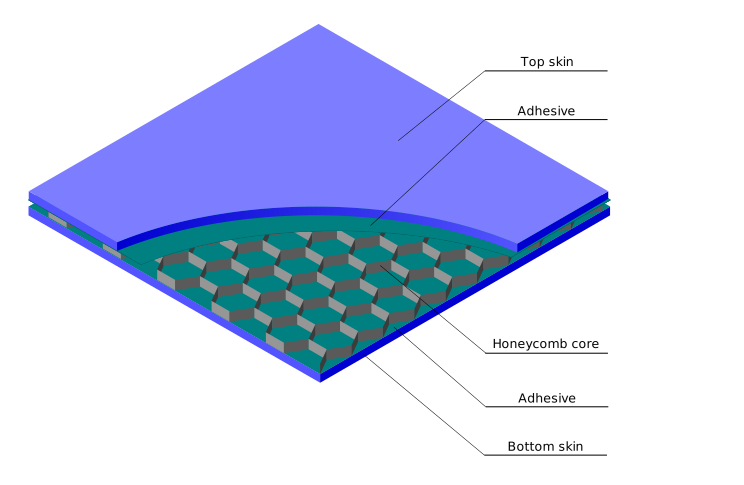
\includegraphics[width=0.95\textwidth]{Intro/honeycomb_plate}
		\caption{
			\label{fig:hcp} Structure of the honeycomb sandwich composite}
		\vspace{-0.5cm}
	\end{center}
\end{figure}

However, various types of damage can occur in these complex structures not found in metal alloy materials. These types of damage include hidden disbonds of the skin and core, delamination of composite skins, or impact damage to the core.
Damage can appear during manufacturing, storage, and operation, so online defect detection methods are required.
Therefore, the increased use of composite materials in the industry has motivated the development of advanced approaches to structural inspections, e.g., methods based on elastic wave propagation had to account for the anisotropic structure of the material.
%% SECTION HEADER /////////////////////////////////////////////////////////////////////////////////////
\section{Structural Health Monitoring}
\label{sec:scm}

%% SECTION CONTENT ////////////////////////////////////////////////////////////////////////////////////
\Ac{shm} is the process of implementing an advanced damage identification strategy for structural or mechanical systems \cite{farrar2007introduction}.
The \ac{shm} systems usually consist of a sensor network, a \ac{dau}, and a central processor.
The \ac{dau} is responsible for collecting the data measured by the sensor network and the intact structure data if used \ac{shm} technique requires it.
A central unit then determines the current state of the structure through signal processing and statistical classification.
\ac{shm} implementation aims to extend the safe life of equipment, use lightweight materials, and reduce manufacturing and operating costs.
For example, the use of composites and adhesive bonding techniques reduces the aircraft's overall weight, thereby reducing fuel consumption \cite{scelsi2011potential}.
\ac{shm} is most commonly found in structures, such as aerospace, civil and mechanical engineering, where damage can have catastrophic consequences.

In his dissertation \cite{rytter1993vibrational}, Rytter classified the \ac{shm} system advancement into the following four levels:
\begin{itemize}
	\item[] \textbf{Level 1}: Detection
	\item[] \textbf{Level 2}: Localization,
	\item[] \textbf{Level 3}: Assessment,
	\item[] \textbf{Level 4}: Consequence.
\end{itemize}
The first level determines if there has been an adverse change in the geometric or material characteristics of the system, and the second level leads to localization of the damage.
The third and fourth level systems determine the size of the flaw and decide whether any maintenance is necessary, respectively.
While existence and location identification can be performed without knowledge of the intact state of the structure, the two last levels require a supervised learning mode \cite{worden2007fundamental}.
%% SECTION HEADER /////////////////////////////////////////////////////////////////////////////////////
\section{Piezoelectric Transducers}
\label{sec:PZT}

%% SECTION CONTENT ////////////////////////////////////////////////////////////////////////////////////
The piezoelectric phenomenon is the generation of an electrical charge on the surface of materials under mechanical deformation in crystalline materials with no inversion symmetry.
The magnitude of the generated charge is proportional to the strain and the direction of polarization.
Those materials also exhibit the opposite effect: a change in size due to an applied electric field.
Piezoelectric materials are widely used in engineering as electroacoustic transducers, high voltage generators and power sources, energy harvesters, micro motors and actuators.
\begin{figure}[H]
	\begin{center}
		\includegraphics{Intro/PZTs}
	\end{center}
	\caption{Various types of piezoelectric transducers \textbf{(a)} circular discs, \textbf{(b)} circular array of the transducers, \textbf{(c)} Smart Layer\textsuperscript{\tiny\textregistered} sensors - piezoelectrics embedded into dielectric film manufactured by Acellent Technologies, Inc.}
	\label{fig:piezo}
\end{figure}
\Acp{pzt}, the acronym derived from the chemical formula of the most commonly used piezoelectric ceramic, i.e. Pb[Zr\(_x\)Ti\(_{1-x}\)]O\(_3\) (lead zirconate titanate), are lightweight, various size and shape structures. 
They can be permanently mounted on the structure surface, embedded within the material, or even be a smart composite material.
In \ac{shm}, they are mainly used in elastic wave propagation, modal analysis, and \ac{emi} methods.
%% SECTION HEADER /////////////////////////////////////////////////////////////////////////////////////
\section{Chosen \acs{shm} techniques using \acsp{pzt}}
\label{sec:techniques}

%% SECTION CONTENT ////////////////////////////////////////////////////////////////////////////////////

\subsection{Guided waves based techniques}


\Acp{gw} are mechanical waves being a superposition of shear and longitudinal waves propagating in a bounded elastic medium, e.g., bars, beams, rods, plates and shells. 
Guided waves are multi-modal and dispersive, i.e. more than one mode travels simultaneously through the medium with the phase velocity depending on the frequency.
Fig.~\ref{fig:dispersion} shows an example of dispersion curves generated by the Dispersion Calculator~\cite{huber2021dispersion} software tool for a 1 \unit{\mm} thick \ac{cfrp} plate in the frequency range 0-2000 \unit{\kHz}.
\Ac{a0} and \ac{s0}, considering the distribution of particle displacements on the upper and lower free surface relative to a central surface, are observed for low frequencies.
The mode shapes are pictured in Fig.~\ref{fig:mode_shape}, with the \ac{s0} particle displacements being dominant in-plane, while the \ac{a0} is dominated by out-of-plane.
Moreover, higher harmonic modes appear over the cut-off frequency, as shown in Fig.~\ref{fig:dispersion}.
\begin{figure}
	\begin{center}
		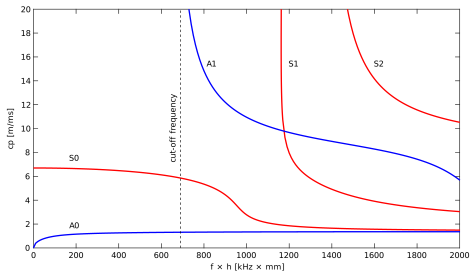
\includegraphics[width=0.95\textwidth]{Intro/dispersion}
	\end{center}
	\caption{Dispersion diagram for a 1 \unit{\mm} \acf{cfrp} plate (adopted from Dispersion Calculator~\cite{huber2021dispersion}). Red and blue solid curves represent symmetric and antisymmetric modes, respectively; a black dashed line indicates the cut-off frequency for higher modes.}
	\label{fig:dispersion}
\end{figure}
\begin{figure}
	\begin{center}
		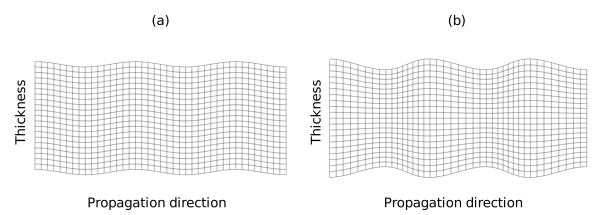
\includegraphics[width=0.95\textwidth]{Intro/mode_shape}
	\end{center}
	\caption{Mode shape of the \textbf{(a)} \acf{a0} and \textbf{(b)} \acf{s0} at 100 \unit{\kHz} for \(\phi\)=\ang{0} in 2 \unit{\mm} composite plate (exported from Dispersion Calculator~\cite{huber2021dispersion}).}
	\label{fig:mode_shape}
\end{figure}

Detection schemes based on \acp{gw} exploit reflection, attenuation, and mode conversion when the propagating wave encounters a discontinuity in the structure \cite{alleyne1992interaction}.
Thus, this technique is efficient in detecting various types of defects, such as delamination \cite{sohn2011delamination,tian2015delamination}, adhesive disbonds \cite{rucka2018damage,balasubramaniam2021ultrasonic}, corrosion changes \cite{alleyne1995long,lowe1998defect}, cracks \cite{tua2004detection,lu2006crack,zima2020detection} and failures occurring in \acp{hsc} \cite{mustapha2011assessment, sikdar2016guided, sikdar2016ultrasonic,radzienski2016assessment, yu2019core}.
Many techniques based on \ac{gw} propagation have been developed for damage detection and localization.
A pitch-catch technique \cite{ihn2008pitch, sikdar2017structural} uses a pair of sensors, one excites, and the other receives a signal.
If the wave encounters a defect between the sensors, it will scatter, and the recorded signal will be distorted.
In the case of the pulse-echo technique \cite{guo1993interaction, kudela2008damage}, there is one sensor that excites the wave and, at the same time, registers possible echoes from the damage.
The damage localization can be determined if the wave speed is known and the time of flight is measured.
The radar principles were utilized in a phased array technique for plate inspection \cite{giurgiutiu2004embedded, ostachowicz2008elastic, kudela2018structural}.
The technique uses an array of transducers, each excited with an appropriate time offset, to focus all the waves at a single grid point of the area to be inspected.
A damage map is determined once the signals are obtained and processed for the entire grid.
Fink proposed a different approach, developing what he called a time-reversal mirror \cite{fink1992time}.
In this method, the wave propagates from one sensor to another, and then after time-reversal and dispersion compensation, the wave is re-emitted to the origin sensor.
The resulting signal will be a mirror image of the forcing signal only if the wave does not encounter damage along the way \cite{park2007time, eremin2016analytically}.

The \acp{pzt} can be used mutually as actuator-receiver pairs or as a single actuator with other types of devices, e.g. \ac{sldv}, \ac{fbg} sensors.
The \acp{pzt} generate high forces with broadband frequency, so methods based on \ac{gw} can detect various damage types of different sizes in a large inspected area.
Moreover, specific algorithms do not require a baseline model, and the method implementation is economically efficient.

\subsection{Electromechanical impedance methods}
\Ac{emi} spectroscopy is also an effective and powerful technique in \ac{shm} for real-time structural damage assessment \cite{park2003overview}.
The basis of this method is the influence of the mechanical impedance of the inspected host structure on the electrical impedance of the \ac{pzt} attached to the structure.
Assuming that the mechanical property of the sensor remains unchanged over the monitoring period, any changes in measurements of the electrical impedance can be considered a difference in the structure stiffness, which in turn can indicate that a defect has occurred.

Fundamentals of the \ac{emi} method were introduced by Liang et al. \cite{liang1994impedance}.
An analytical model of a \ac{pzt} actuator bonded to one end of a single degree of freedom mass-spring-damper system was presented in this pioneering work.
In the early papers, the authors adopted quasi-static sensor approximation until  Giurgiutiu and Zagrai \cite{giurgiutiu2000characterization} derived an expression where the sensor dynamic was incorporated.
The dynamics of a single \ac{pzt} with various boundary conditions (free, clamped and elastically constrained) and sensor attached to a beam were considered.
Further investigation was performed for the sensor bonded to the host structures \cite{zagrai2001electro, giurgiutiu2005damage}.
Damage detection is realised by comparing the state of the structure with the reference state using overall statistical damage indices, e.g., the \ac{rmsd}, the \ac{mapd}, \ac{ccd} and \ac{pnn}.
Malinowski et al. \cite{malinowski2014characterisation, malinowski2015use} investigated the effects of \ac{emi} changes related to the state of the adhesive layer between two composite plates.
The technique has been used to evaluate weak bonds due to inadequate adhesive curing temperature, release agent and moisture contamination. This type of damage is not detectable using the method based on \ac{gw} propagation.
Experimental testing was conducted on weakened samples and compared with a reference.
The \ac{rms} of the conductance in the range of 3-5 MHz and the first thickness resonant frequency shift were considered for bond-line assessment.

An and Sohn \cite{an2012integrated} proposed a new damage detection technique that combines \ac{emi} and \ac{gw} advantages.
In the method, measured admittance characteristic is separated into two parts: active and passive.
\Ac{di} is a weighted sum of two indicators obtained from \ac{gw} signal and active admittance.
Because passive impedance is only sensitive to temperature variation, it is used for temperature compensation on both mentioned signals.
Instead of two \acp{di}, Sevillano et al. \cite{sevillano2016damage} proposed more integrated \ac{di} based on the electromechanical power dissipation of the \ac{pzt} sensor.

The \ac{emi} technique can detect damage, such as delamination or cracks, but is also sensitive to changes, such as weak bonds, which the \ac{gw} method is ineffective at detecting.
However, the \ac{emi} is a local method for the high frequency.
Giurgiutiu et al. \cite{giurgiutiu2001electro} obtained consistent results for crack detection in distances up to 40 \unit{\mm} from the sensor in the frequency range 300-450 \unit{\kHz}. 
This method is also sensitive to environmental conditions such as temperature and humidity fluctuations\cite{bhalla2002practical} or loading variations \cite{lim2011impedance}.

%\subsection{Modal analysis techniques}
%% SECTION HEADER /////////////////////////////////////////////////////////////////////////////////////
\section{Challenges in Damage Assessment in the SCS}
\label{sec:challenges}

%% SECTION CONTENT ////////////////////////////////////////////////////////////////////////////////////



\section{Conclusions}
\label{sec:conclusionsIntro}

%% SECTION CONTENT ////////////////////////////////////////////////////////////////////////////////////
In the Introduction, a brief overview of problems undertaken in the dissertation has been presented, i.e., composite materials, construction and their applications;  definition of the \ac{shm} and application of \ac{pzt} sensors in damage detection; and challenges in \ac{gw} propagation modelling for damage severity assessment in the \acp{hsc}.
The most relevant issues address to:
\begin{itemize}
	\item flexibility to model complex structure of the honeycomb core;
	\item time efficiency due to the high number of \ac{dof} of the model;
	\item possibility to parallel calculation on the \ac{gpu}.
\end{itemize}
The literature review revealed the need for a practical tool for damage size estimation in the \acp{hsc} to increase the safe usage of the engineering structures made of composites. 
Therefore, in the dissertation, I have tried to develop an effective way to determine the function of the effect of damage size on elastic wave propagation.

% Set page numbering to arabic the first time we commence a chapter.
% This is required to get the page numbering correct.
\pagenumbering{arabic}

% Note that the text in the [] brackets is the one that will
% appear in the table of contents, whilst the text in the {}
% brackets will appear in the main thesis.

%% CHAPTER HEADER /////////////////////////////////////////////////////////////////////////////////////
\chapter[Problem Statement]{Problem Statement}
\label{ch:problem}

%% CHAPTER INTRODUCTION ////////////////////////////////////////////////////////////////////////////////////

%% INCLUDE SECTIONS ////////////////////////////////////////////////////////////////////////////////////

Composite materials are used as structural components whose failure can have catastrophic consequences.
Although \ac{gw} based methods are promising for damage identification and localization, they have not been widely reported to estimate the failure size.
A better understanding of the effect of damage on elastic wave propagation in \acp{hsc} will allow the development of robust and practical tools to evaluate this structure.

The principal aim of this dissertation was to propose a new approach for the severity of damage identification in the \ac{hsc} employing the \ac{pzt} sensors.
The essence of the method is the determination of damage influence function on characteristic parameters of the propagating waves in the structure.
This function was defined using a numerical model developed by the \ac{sem}.

Initially, the model is prepared for the pristine sample under various operating conditions such as ambient temperature.
Then parametric simulations for different damage scenarios are performed.
The \ac{madif} is determined based on the obtained results. 
This function determines the flaw size depending on the \acp{pzt} response.
Damage is considered to be a debonding between the core and the skin. 
The following objectives of the dissertation are:
\begin{itemize}
	\item Develop a robust and efficient numerical model of the propagating \ac{gw} in the \ac{hsc} under varying ambient temperatures.
	\item Validate the model experimentally.
	\item Determine the \ac{madif} to define damage influence on the propagating waves.
	\item Investigate the structure experimentally under varied temperature conditions.
	\item Propose a framework of damage detection based on the \ac{madif}.
\end{itemize}

The imposed objectives lead to the proof of the thesis that it is possible to determine the function of damage severity in \acp{hsc} by numerical simulations.

Chapter \ref{ch:method} presents the methods for developing a model-assisted damage severity assessment scheme.

Chapter \ref{ch:sem} gives a theoretical background of the \ac{sem} for \ac{gw} propagation.
It includes mass, stiffness and damping matrices for 2D and 3D formulation; interface coupling algorithm; time integration scheme; and parallel implementation for GPU calculation.

Chapter \ref{ch:simulation} provides the details of the sample configuration for the full geometry and homogenized core models. The individual sample component grids, the signal parameters, and the damage model are presented.

The simulations and experimental validation results are presented in Chapter \ref{ch:validation}.

Chapter \ref{ch:tempEffects} includes the analysis of the GW propagation under variable temperature conditions.

The crucial part of the dissertation appears in Chapter \ref{ch:severity}. Based on the simulations performed and their validation experimentally, the function of the damage size effect on the elastic wave propagation in \ac{hsc} is revealed, termed \ac{madif}.

The conclusion of the dissertation and final remarks are provided in Chapter \ref{ch:conclusions}.


% Note that the text in the [] brackets is the one that will
% appear in the table of contents, whilst the text in the {}
% brackets will appear in the main thesis.

%% CHAPTER HEADER /////////////////////////////////////////////////////////////////////////////////////
\chapter[Concept of the Method]{Concept of the Method}
\label{ch:method}

%% CHAPTER INTRODUCTION ///////////////////////////////////////////////////////////////////////////////


%% INCLUDE SECTIONS ///////////////////////////////////////////////////////////////////////////////////

%% SECTION HEADER /////////////////////////////////////////////////////////////////////////////////////
\section{Modeling of the \acs{gw} propagation in the \acsp{hsc}}
\label{sec:modelling}

%% SECTION CONTENT ////////////////////////////////////////////////////////////////////////////////////

%% SUBSECTION HEADER //////////////////////////////////////////////////////////////////////////////////

In the dissertation, the \ac{hsc} composed of an aluminium honeycomb core and the skin made of \ac{cfrp} is assumed for further analysis.
The most common numerical modeling of the phenomenon of \ac{gw} in the \acp{hsc} found in the literature is a calculation of the effective material properties of the honeycomb structure \cite{baid2015dispersion, mustapha2014leaky, qi2008ultrasonic,  shi1995derivation, sikdar2016guided}.
The properties are obtained from the analytical \cite{gibson1982mechanics, malek2015effective} or the \ac{fem} \cite{catapano2014multi, chen2014analysis} analysis of the honeycomb \ac{rve}.
A comprehensive literature review on the homogenisation of the honeycomb structure is presented in the work of Ahmed \cite{ahmed2019homogenization}.
Replacing the core geometry with a homogeneous material has many advantages.
First and foremost, it simplifies the domain mesh so that convergence of the solution requires fewer working memory resources and increases the value of the critical time step.
In addition, the wave propagation velocity determined by the simulation is in good agreement with the experiment.

However, this method cannot adequately represent the phenomenon of propagating wave interaction in honeycomb cells.
It causes the signal energy not to dissipate as it would in a real structure.
A more precise model is the \ac{fcgm}. 
Ruzzene et al. presented a parametric study to evaluate the dynamic behavior of the honeycomb and cellular structures through the \ac{fem} and the application of the theory of periodic structures \cite{ruzzene2003wave}.
Recently, the simulations of the wave propagation in the \acp{hsc} have been conducted with commercially available finite element codes~\cite{song2009guided, hosseini2013numerical, tian2015wavenumber, zhao2018wave}.

While the \ac{fem} based modelling of \ac{gw} requires a significant amount of memory and is time-consuming, this method becomes inefficient in the case of \ac{fcgm}.
Kudela increased the computational efficiency with the model based on the time-domain \ac{sem} \cite{kudela2016parallel}.
In addition, the algorithm has been adapted for parallel computing on the \ac{gpu}, making the simulations 14 times faster than on the \ac{cpu}.
However, this approach has two major drawbacks. One is employing solid elements with three \acp{dof} at each node to model the core walls. As a result, a \numproduct{179 x 160} \unit{\square\mm} sandwich panel has over 1.5 million \acp{dof}.
Secondly, no \ac{pzt} sensors were considered in the simulation, so a concentrated force was used to generate the \ac{gw}.
To attach the transducers, the grids of the sensor and the host plate must coincide or use an interface between them. 

The disadvantages of existing modelling methods, motivated me to propose a new model of the \ac{hsc}.
In the proposed model, the core of the plate consists of \ac{2d} elements, one per cell wall.
Since the neutral plane of the elements is oriented differently concerning the global coordinate system, the local displacements vector has to be transformed accordingly.
The skin model is developed according to the laminate theory presented by Vinson and Sierakowski \cite{vinson1993behavior}.
In addition, two interfaces are used to connect the individual \ac{hsc} components.
One with the non-matching grid was developed to join the sensors with the panel.
It was done with the novel method based on the element shape functions described in Chapter \ref{ch:sem}.
The core and skin connection was implemented with a perfect matching interface.
To the best of my knowledge, the presented model has not been implemented yet for the \acp{hsc}.

The parametric study conducted in the dissertation leads to the determination of a \ac{madif}, which defines the influence of the composite defect size on wave propagation.
In this case, the defect is assumed to be a disbond between the skin and the core.
%% SECTION HEADER /////////////////////////////////////////////////////////////////////////////////////
\section{Temperature Effect on the GW Propagation}
\label{sec:temp}

%% SECTION CONTENT ////////////////////////////////////////////////////////////////////////////////////

%% SUBSECTION HEADER //////////////////////////////////////////////////////////////////////////////////
In order to carry out the temperature dependent SE simulation and semi-analytical analysis of Lamb wave propagation in the \acp{hsc}, the elastic modulus of \acp{hsc} layers are calculated as per the methodology described in \cite{chamis1983simplified,salamone2009guided}. The calculation is done for a range of temperature (+50\(^{\circ}\)C to -50\(^{\circ}\)) generally occurred in practical operating scenarios. The obtained temperature-dependent elastic properties (E11 = E22, E33, G12, G13 = G23) for composite laminate and adhesive (E, G) are presented in Figure 7 and Figure 8, respectively.

In this model \cite{salamone2009guided}, reduction of Young’s modulus of resin \(E_m\) with variation in temperature is assumed as:
\begin{eqnarray}
	E_m(T)=F_m E_{rm},
	\label{eq:factor_temp}
\end{eqnarray}
where \(E_{rm}\) is the Young’s Modulus of resin at the reference temperature and \(F_m\) is the temperature degradation factor as proposed in \cite{chamis1983simplified}:
\begin{eqnarray}
F_m=\sqrt{\frac{T_{g0}-T}{T_{g0}-T_r}},
\label{eq:em_temp}
\end{eqnarray}
where \(T_{g0}\) is the glass transition temperature and \(T_r\) is the reference temperature. In the study, the value of \(T_{g0}=215^{\circ}C\) and \(T_r=20^{\circ}C\) is selected from Table 2 in \cite{chamis1983simplified}. 

%% SECTION HEADER /////////////////////////////////////////////////////////////////////////////////////
\section{Model-assisted damage severity assessment}
\label{sec:madif}

%% SECTION CONTENT ////////////////////////////////////////////////////////////////////////////////////

%% SUBSECTION HEADER //////////////////////////////////////////////////////////////////////////////////
The process of determining the damage size is shown in the flowchart in Figure \ref{fig:Flowchart} \cite{fiborek2021model}.
Before inspecting a given \ac{hsc} panel, a numerical analysis has to be performed to determine a function that describes the effect of damage on wave propagation.
Then the model is subjected to experimental validation.
If the simulation results did not agree with the measured results, the material parameters of the components were adjusted.
In the dissertation, the \ac{cfrp} volume fraction of reinforcing fibres was adjusted to determine a wave velocity \cite{kudela2007modelling} and a damping coefficient of the skin to set the magnitude of the registered signals \cite{wandowski2017guided}.
\begin{figure}[!tbh]
	\begin{center}
		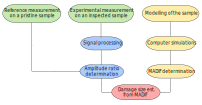
\includegraphics[width=0.95\textwidth]{Chapter_3/flowchart}
	\end{center}
	\caption{A flowchart representing the process for damage size estimation}
	\label{fig:Flowchart}
\end{figure}
\clearpage
When the structure model was developed, several computer simulations for various damage sizes were conducted to determine the \ac{madif}, a cornerstone of the dissertation. This function determines the severity of \ac{hsc} damage based on the signal received by the sensor.
Several excitation signals and damage indices were considered to select the best \ac{madif}.
The selection criterion was the monotonicity and the function slope over the considered range of the damage size. Then, the damage magnitude was obtained from the \ac{madif} for the measured signal and normalised to the reference one.
%% SECTION HEADER /////////////////////////////////////////////////////////////////////////////////////
\section{Conclusions}
\label{sec:conclusionsMethod}

%% SECTION CONTENT ////////////////////////////////////////////////////////////////////////////////////




% Note that the text in the [] brackets is the one that will
% appear in the table of contents, whilst the text in the {}
% brackets will appear in the main thesis.

%% CHAPTER HEADER /////////////////////////////////////////////////////////////////////////////////////
\chapter{Formulation of the Time-Domain Spectral Element Method}
\label{ch:sem}
%% CHAPTER INTRODUCTION ///////////////////////////////////////////////////////////////////////////////
The comprehensive formulation of the \ac{sem}-based numerical model is presented in the Chapter.
It includes shape function definition, numerical integration in the scheme of the \ac{gll}, determination of the structural matrices for solid and first-order shear deformation theory elements and electromechanical coupling for the \acp{pzt}.
The non-matching interface was introduced with the novel approach based on the element shape functions.
These components were combined to implement the \ac{sem} for the honeycomb structure with the \ac{fcgm}, which has not been found in the literature before.

%% INCLUDE SECTIONS ///////////////////////////////////////////////////////////////////////////////////
%% SECTION HEADER /////////////////////////////////////////////////////////////////////////////////////
\section{High order polynomial interpolation and the \acl{gll} integration scheme}
\label{sec:sem}

%% SECTION CONTENT ////////////////////////////////////////////////////////////////////////////////////

The \ac{sem} is similar to the \ac{fem}.
The similarity of both methods lies in the fact that considered domain is divided into non-overlapping finite elements, and external forces and arbitrary boundary conditions are imposed in the particular nodes.
The main difference between those methods is a selection of the shape function \( N=N(\xi )\), pictured in Figure~\ref{fig:shape}, which is interpolated by a Lagrange polynomial that passes through the element nodes.
The nodes are localised on the endpoint of an interval, \(\xi\in[-1,1]\), and the roots of the first derivative of Legendre polynomial \(\mathcal{P}\) of degree \(p\):
\begin{eqnarray}
	(1-\xi^2)\mathcal{P}'_{p}(\xi)=0.
	\label{eq:nodes}
	\nomtypeD[x]{\( \xi, \eta, \zeta \)}{Local coordinates}{}
	\nomtypeD[w]{\(w\)}{Weighting factor}{}
\end{eqnarray}
The approximation of an integral over the elements is achieved according to the \ac{gll} rule at points coinciding with the element nodes. The integration weights \(w=w(\xi)\) equal
\begin{eqnarray}
	{w(\xi)} = \frac{2}{p(p+1)(\mathcal{P}_{p}(\xi))^2}.
	\label{eq:weight}
\end{eqnarray}

The shape functions and the weights for \ac{2d} or \ac{3d} elements are obtained by the Kronecker product of vectors of individual axes, denoted by \(\otimes\) as follows:
\begin{eqnarray}
	\begin{array}{rcl}
	N(\xi,\eta) & = & N(\xi)\otimes N(\eta),\\
	N(\xi,\eta,\zeta) & = & N(\xi)\otimes N(\eta)\otimes N(\zeta),
	\end{array}
\label{eq:shape_functions}
\nomtypeD[N]{$N$}{Shape function}{}
\end{eqnarray}
\begin{eqnarray}
	\begin{array}{rcl}
	w(\xi,\eta) & = & w(\xi)\otimes w(\eta),\\
	w(\xi,\eta,\zeta) & = & w(\xi)\otimes w(\eta)\otimes w(\zeta).
	\end{array}
	\label{eq:weights}
\end{eqnarray}
\begin{figure}[H]
	\begin{center}
		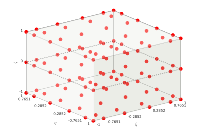
\includegraphics[width=0.95\textwidth]{Chapter_4/shape_function}
	\end{center}
	\caption{Shape functions based on fifth-order polynomial interpolation}
	\label{fig:shape}
\end{figure}

The derivation of the equation of motion is given in \cite{ostachowicz2011guided}, and it is defined as
\begin{eqnarray}
	\label{eq:motion}
	\textbf{M} \ddot{\textbf{d}} + \textbf{D} \dot{\textbf{d}} + \textbf{K} \textbf{d} = \textbf{f}_{ext},
	\nomtypeR[M]{$\textbf{M}$}{Mass matrix}{}{\unit{\kg}}%
	\nomtypeR[D]{$\textbf{D}$}{Damping matrix}{}{\unit[per-mode = symbol]{\newton\second \per \meter}}%
	\nomtypeR[K]{$\textbf{K}$}{Stiffness matrix}{}{\unit[per-mode = symbol]{\newton\per\metre}}%
	\nomtypeR[force_ext]{$\textbf{f}_{ext}$}{External force vector}{}{\unit{\newton}}%
	\nomtypeR[d]{$\textbf{d}$}{Displacements vector}{}{\unit{\meter}}%
\end{eqnarray}
where \textbf{d} is the displacements vector; \textbf{M}, \textbf{D} and \textbf{K} are the structural mass, damping and stiffness matrices, respectively; \textbf{F}$_{ext}$ is the external forces vector; \((\dot{\ })=\frac{\partial}{\partial t}\).
The construction of the structural matrices is similar to the classical approach in \ac{fem}.

The most significant advantage of this method is the fast convergence of the equation of motion.
It is achieved for six nodes per wavelength, while at least fifteen nodes are needed in the case of linear elements in classic \ac{fem}~\cite{wee2017simulating}.
In addition, the mass matrix is diagonal when using the \ac{gll} approach and solid elements or elements based on first-order shear deformation theory.

%% SECTION HEADER /////////////////////////////////////////////////////////////////////////////////////
\section{2D Spectral Modelling}
\label{sec:2Dmodel}

%% SECTION CONTENT ////////////////////////////////////////////////////////////////////////////////////

According to the first-order shear deformation theory~\cite{reissner1945effect, mindlin1951influence}, the displacement field is expressed as:
\begin{eqnarray}
	\left \{ \begin{array}{c}
		\textbf{u}^e(\xi,\eta) \\
		\textbf{v}^e(\xi,\eta) \\
		\textbf{w}^e(\xi,\eta)
	\end{array} \right\} = 
	\left \{ \begin{array}{c}
		\textbf{u}_0^e(\xi,\eta) + z\boldsymbol{\varphi}_x^e(\xi,\eta)\\
		\textbf{v}_0^e(\xi,\eta) + z\boldsymbol{\varphi}_y^e(\xi,\eta)\\
		\textbf{w}_0^e(\xi,\eta) \\
	\end{array} \right\},
\end{eqnarray}
where \(\textbf{u}_0^e\), \(\textbf{v}_0^e\) and \(\textbf{w}_0^e\) are nodal displacements, \(\boldsymbol{\varphi}_x^e\), \(\boldsymbol{\varphi}_y^e\) are the rotations of the normal to the mid-plane with respect to the axes \textit{x} and \textit{y}, respectively.
\begin{eqnarray}
	\left \{\begin{array}{c}
		\textbf{u}_0^e(\xi,\eta) \\
		\textbf{v}_0^e(\xi,\eta) \\
		\textbf{w}_0^e(\xi,\eta) \\
		\boldsymbol{\varphi}_x^e(\xi,\eta) \\
		\boldsymbol{\varphi}_y^e(\xi,\eta)
	\end{array} \right\}
	= \textbf{N}^e(\xi,\eta)\widehat{\textbf{d}}^e
	= \sum_{n=1}^q\sum_{m=1}^p\textbf{N}_m^e(\xi)\textbf{N}_n^e(\eta)
	\left \{ \begin{array}{c}
		\widehat{\textbf{u}}_0^e \\
		\widehat{\textbf{v}}_0^e \\
		\widehat{\textbf{w}}_0^e \\
		\widehat{\boldsymbol{\varphi}}_x^e \\
		\widehat{\boldsymbol{\varphi}}_y^e
	\end{array} \right \}.
\end{eqnarray}

The nodal bending strain--displacement relations are given in the form:
\begin{eqnarray}
	\boldsymbol{\epsilon}_b^e =
	\textbf{B}_b^e\widehat{\textbf{d}}^e = 
	\left [
	\begin{array}{ccccc}
		\frac{\partial N^e}{\partial x} & 0 & 0 & 0 & 0\\
		0 & \frac{\partial N^e}{\partial y} & 0 & 0 & 0\\
		\frac{\partial N^e}{\partial y} & \frac{\partial N^e}{\partial x} & 0 & 0 & 0\\
		0 & 0 & 0 & -\frac{\partial N^e}{\partial x} & 0\\
		0 & 0 & 0 & 0 & -\frac{\partial N^e}{\partial y}\\
		0 & 0 & 0 & -\frac{\partial N^e}{\partial y} & -\frac{\partial N^e}{\partial x}
	\end{array} \right]
	\left \{ \begin{array}{c}
		\widehat{\textbf{u}}_0^e \\
		\widehat{\textbf{v}}_0^e \\
		\widehat{\textbf{w}}_0^e \\
		\widehat{\boldsymbol{\varphi}}_x^e \\
		\widehat{\boldsymbol{\varphi}}_y^e
	\end{array} \right\}.
\end{eqnarray}

The nodal shear strain--displacement relations are given in the form:
\begin{eqnarray}
	\boldsymbol{\epsilon}_s^e =
	\textbf{B}_s^e\widehat{\textbf{d}}^e = 
	\left [
	\begin{array}{ccccc}
		0 & 0 & \frac{\partial N^e}{\partial y} & -1 & 0\\
		0 & 0 & \frac{\partial N^e}{\partial y} & 0 & -1
	\end{array} \right]
	\left \{ \begin{array}{c}
		\widehat{\textbf{u}}_0^e \\
		\widehat{\textbf{v}}_0^e \\
		\widehat{\textbf{w}}_0^e \\
		\boldsymbol{\varphi}_x^e \\
		\boldsymbol{\varphi}_y^e
	\end{array} \right\}.
\end{eqnarray}
%% SECTION HEADER /////////////////////////////////////////////////////////////////////////////////////
\section{3D Spectral Modelling}
\label{sec:3Dmodel}

%% SECTION CONTENT ////////////////////////////////////////////////////////////////////////////////////
The displacement vector of the \ac{3d} element is composed of three translational displacements defined as:
\begin{eqnarray}
	\left \{ \begin{array}{c}
		\textbf{u}^e(\xi,\eta,\zeta) \\
		\textbf{v}^e(\xi,\eta,\zeta) \\
		\textbf{w}^e(\xi,\eta,\zeta)
	\end{array} \right\}
	= \textbf{N}^e(\xi,\eta, \zeta)\widehat{\textbf{d}}^e
	= \sum_{l=1}^r\sum_{n=1}^q\sum_{m=1}^p\textbf{N}_m^e(\xi)\textbf{N}_n^e(\eta)\textbf{N}_l^e(\zeta)
	\left \{ \begin{array}{c}
		\widehat{\textbf{u}}^e(\xi_m,\eta_n,\zeta_l) \\
		\widehat{\textbf{v}}^e(\xi_m,\eta_n,\zeta_l) \\
		\widehat{\textbf{w}}^e(\xi_m,\eta_n,\zeta_l)
	\end{array} \right\},
	\label{eq:3D_displ}
\end{eqnarray}
where \(\widehat{\textbf{u}}^e\), \(\widehat{\textbf{v}}^e\) and 
\(\widehat{\textbf{w}}^e\) are displacements of the element nodes in \(\xi,\eta\) and \(\zeta\) direction.

The nodal strain--displacement relations are given as \cite{kudela20093d}:
\begin{eqnarray}
	\boldsymbol{\epsilon}^e=\textbf{B}_{d}^e\widehat{\textbf{d}}^e=
	\left [
	\begin{array}{ccc}
		\frac{\partial N^e}{\partial x} & 0 & 0\\
		0 & \frac{\partial N^e}{\partial y} & 0\\
		0 & 0 & \frac{\partial N^e}{\partial z}\\
		0 & \frac{\partial N^e}{\partial z} & \frac{\partial N^e}{\partial y}\\
		\frac{\partial N^e}{\partial z} & 0 & \frac{\partial N^e}{\partial x}\\
		\frac{\partial N^e}{\partial y} & \frac{\partial N^e}{\partial x} & 0
	\end{array} \right]
	\left \{ \begin{array}{c}
		\widehat{\textbf{u}}^e \\
		\widehat{\textbf{v}}^e \\
		\widehat{\textbf{w}}^e
	\end{array} \right\}.
\end{eqnarray}
The formulae of the structural matrices for 3D elements are:
\begin{eqnarray}
	\textbf{M}_{dd}^e & = & \int_{V_e}\textbf{N}^T\rho \textbf{N} \diff V_e,\\
	\textbf{K}_{dd}^e & = & \int_{V_e}{\textbf{B}_d^e}^T\textbf{C}\textbf{B}_d^e \diff V_e,
\end{eqnarray}
where \textbf{C} is the stiffness tensor, \(\rho\) is mass density, and \(V_e\) is the element volume.
%% SECTION HEADER /////////////////////////////////////////////////////////////////////////////////////
\section{\Acs{pzt} modelling}
\label{sec:PZTmodel}

%% SECTION CONTENT ////////////////////////////////////////////////////////////////////////////////////
The electromechanical coupling is governed by the linear constitutive equation of piezoelectric material according to~\cite{giurgiutiu2009micromechatronics, rekatsinas2017cubic}, and this is defined as:
\begin{eqnarray}
	\left [ 
	\begin {array}{c}
	\boldsymbol{\sigma}\\
	\widetilde{\textbf{D}}
\end{array}\right ]=
\left [ 
\begin{array}{cc}
	\textbf{c}^E & -\textbf{e}^{\mathrm{T}} \\
	\textbf{e} & \epsilon^S 
\end{array} \right ]
\left[ 
\begin{array}{c}
	\boldsymbol{\varepsilon}\\
	\widetilde{\textbf{E}} 
\end{array} \right ],
\label{eq:elecmechcoupling}
\end{eqnarray}
\nomtypeR[Ep]{$\widetilde{\textbf{E}} $}{Electric field}{\(-\textbf{B}\,\boldsymbol{\phi}\)}{\unit[per-mode=symbol]{\newton\per\coulomb}}%
\nomtypeR[Dp]{$\widetilde{\textbf{D}} $}{Electric charge density displacement}{-}{\unit[per-mode=symbol]{\coulomb\per\square\metre}}%
\nomtypeG[phip]{$\boldsymbol{\phi}$}{Electric potential vector}{-}{\unit{\volt}}%
\nomtypeG[sigma]{$\boldsymbol{\sigma}$}{Stress tensor}{\(\textbf{c}\,\boldsymbol{\varepsilon}\)}{\unit{\pascal}}%
where \(\boldsymbol{\sigma}\) is the stress components, \(\textbf{c}^E\) is the stiffness coefficient matrix measured at zero electric field, \textbf{e} is the piezoelectric coupling tensor, \(\boldsymbol{\epsilon}^S\) is the electric permittivity measured at zero strain, and \(\widetilde{\textbf{E}}\) and \(\widetilde{\textbf{D}}\) are the electric field and electric charge density displacement.
The electric field of the element is defined as:
\begin{eqnarray}
\widetilde{\textbf{E}}^e=-\textbf{B}_\phi^e \widehat{\boldsymbol{\phi}}^e = \left[ \begin{array}{c}
	\frac{\partial N^e}{\partial \xi}\\
	\frac{\partial N^e}{\partial \eta}\\
	\frac{\partial N^e}{\partial \zeta}
\end{array} \right] \widehat{\boldsymbol{\phi}}^e,
\end{eqnarray}
where \(\widehat{\boldsymbol{\phi}}^e\) is a nodal voltage of the transducer. The \ac{sem} formulation of the governing equation (\ref{eq:elecmechcoupling}) is defined as:
\begin{eqnarray}
	\left [\begin{array}{cc}
		\textbf{M}_{dd} & \textbf{0}\\
		\textbf{0} & \textbf{0}
	\end{array}\right]
	\left \{\begin{array}{c}
		\widehat{\ddot{\textbf{d}}} \\
		\textbf{0}
	\end{array}\right \} +
	\left [\begin{array}{cc}
		\textbf{K}_{dd} & \textbf{K}_{d \phi}\\
		\textbf{K}_{d \phi}^{\mathrm{T}} & \textbf{K}_{\phi \phi}
	\end{array}\right]
	\left \{\begin{array}{c}
		\widehat{\textbf{d}} \\
		\widehat{\boldsymbol{\phi}}
	\end{array}\right \}  = 
	\left \{\begin{array}{c}
		\textbf{0}\\
		\widehat{\textbf{Q}}
	\end{array}\right \},
	\label{eq:pzt_sem}
\end{eqnarray}
\nomtypeR[Q]{$\textbf{Q}$}{Charge vector}{-}{\unit{\coulomb}}%
where \(\widehat{\textbf{Q}}\) is the nodal charge vector.
The mass and stiffness matrices are defined according to \ac{3d} model from section \ref{sec:3Dmodel}.
The piezoelectric coupling matrix \(\textbf{K}_{\phi \phi}^e\) and the dielectric permittivity matrix \(\textbf{K}_{d \phi}^e\) are defined as:
\begin{eqnarray}
	\textbf{K}_{d\phi}^e & = & \int_{V_e}{\textbf{B}_d^e}^{\mathrm{T}}\textbf{e}^{\mathrm{T}} \textbf{B}_{\phi}^e \diff V_e,\\
	\textbf{K}_{\phi \phi}^e & = & -\int_{V_e}{\textbf{B}_{\phi}^e}^{\mathrm{T}} 
	{\textbf{\(\epsilon\)}^S}^{\mathrm{T}} \textbf{B}_{\phi}^e \diff V_e.
\end{eqnarray}

If a vector \(\textbf{b}\) contains list of consecutive boundary nodes (corresponding to electrodes) and a vector \(\textbf{a}\) contains lists of consecutive active nodes (remaining nodes) of the \ac{pzt}, the electrical potential vector and the charge vector can be rewritten as:
\begin{eqnarray}
	\widehat{\boldsymbol{\phi}} & = & \left \{\begin{array}{cc}
		\widehat{\boldsymbol{\phi}}(\textbf{b}) &
		\widehat{\boldsymbol{\phi}}(\textbf{a})
	\end{array}\right \}^{\mathrm{T}},\\
	\widehat{\textbf{Q}} & = & \left \{\begin{array}{cc}
		\widehat{\textbf{Q}}(\textbf{b}) & \textbf{0}
	\end{array}\right \}^{\mathrm{T}}.
	\label{eq:phi_Q}
\end{eqnarray}
Then, piezoelectric part of Eq.~(\ref{eq:pzt_sem}) is expressed as:
\begin{eqnarray}
	\begin{split}
		\left [\begin{array}{cc}
			\textbf{K}_{d \phi}(:,\textbf{b}) &
			\textbf{K}_{d \phi}(:,\textbf{a})
		\end{array}\right]^{\mathrm{T}}
		\widehat{\textbf{d}} & +
		\left [\begin{array}{cc}
			\textbf{K}_{\phi \phi}(\textbf{b},\textbf{b}) & \textbf{K}_{\phi 		\phi}(\textbf{b},\textbf{a})\\
			\textbf{K}_{\phi \phi}(\textbf{a},\textbf{b}) & \textbf{K}_{\phi \phi}(\textbf{a},\textbf{a})
		\end{array}\right]
		\left \{\begin{array}{c}
			\widehat{\boldsymbol{\phi}}(\textbf{b}) \\
			\widehat{\boldsymbol{\phi}}(\textbf{a})
		\end{array}\right \}\\ 
		& = \left \{\begin{array}{c}
			\widehat{\textbf{Q}}(\textbf{b}) \\
			\textbf{0}
		\end{array}\right \},
	\end{split}
	\label{eq:pztboundary}
\end{eqnarray}
where the notation \(\textbf{K}(\textbf{r},\textbf{c})\) uses vectors \(\textbf{r}\) and \(\textbf{c}\) to extract rows and columns from the matrix \(\textbf{K}\), respectively, and \((:)\) means all rows or columns of \(\textbf{K}\).
The electrical potential of the free nodes can be extracted from Eq.~(\ref{eq:pztboundary}):
\begin{eqnarray}
	\widehat{\boldsymbol{\phi}}(\textbf{a}) = -\textbf{K}_{\phi\phi}^{-1}(\textbf{a},\textbf{a})\left[\textbf{K}_{\phi d}(\textbf{a},:) \widehat{\textbf{d}} + \textbf{K}_{\phi\phi}(\textbf{a},\textbf{b})\widehat{\boldsymbol{\phi}}(\textbf{b}) \right].
	\label{eq:freePotetial}
\end{eqnarray}
If the \ac{pzt} acts as an actuator, the electrical potential of the electrode nodes has the values of the applied signal.
As one of the electrodes is grounded, the potential is zero.
Therefore, the potential vector can be written as:
\begin{eqnarray}
	\widehat{\boldsymbol{\phi}}(\textbf{b}) = \left \{\begin{array}{cc}
		\widehat{\boldsymbol{\phi}}(\textbf{b}_v) &
		\widehat{\boldsymbol{\phi}}(\textbf{b}_g)
	\end{array}\right \}^{\mathrm{T}}=\left \{\begin{array}{cc}
	\textbf{V}(t) & \textbf{0}
	\end{array}\right \}^{\mathrm{T}},
	\label{eq:phi_V}
\end{eqnarray}
where \(\textbf{b}_v\) is a list of nodes of the applied electrode and \(\textbf{b}_g\) is a list of nodes of the grounded electrode.
Substituting Eq. (\ref{eq:phi_V}) into Eq. (\ref{eq:freePotetial}) and Eq. (\ref{eq:pztboundary}), induced stiffness of the actuator is obtained:
\begin{eqnarray}
	\textbf{K}_{a}=-\textbf{K}_{d\phi}(:,\textbf{a})\,\textbf{K}_{\phi \phi}^{-1}(\textbf{a},\textbf{a})\,\textbf{K}_{\phi \phi} (\textbf{a},\textbf{b}).
\end{eqnarray}
Hence, the equivalent mechanical force vector of the applied voltage of the piezoelectric actuator equals:
\begin{eqnarray}
	\widehat{\textbf{f}}_{a}=-\textbf{K}_{a}\,\widehat{\boldsymbol{\phi}}(\textbf{b}).
	\label{eq:f_act}
\end{eqnarray}
\nomtypeR[force_act]{$\textbf{f}_{a}$}{Actuator equivalent force vector}{\(-\textbf{K}_a\,\boldsymbol{\phi}(b)\)}{\unit{\newton}}%
In the case of the open circuit sensor one electrode is grounded so the electric potential of the free nodes becomes as:
\begin{eqnarray}
	\widehat{\boldsymbol{\phi}}(\textbf{a}) = -\textbf{K}_{\phi\phi}^{-1}(\textbf{a},\textbf{a})\,\textbf{K}_{\phi d}(\textbf{a},:)\,\widehat{\textbf{d}}.
	\label{eq:sensorPotetial}
\end{eqnarray}
The induced stiffness of the sensor can be written as:
\begin{eqnarray} \textbf{K}_s=\textbf{K}_{d \phi}(:,\textbf{a})\,\textbf{K}_{\phi \phi}^{-1} (\textbf{a},\textbf{a})\,\textbf{K}_{\phi d}(\textbf{a},:).
\end{eqnarray}
To obtain the sensor response, the nodal electric potential must be integrated over the electrode surface as follow:
\begin{eqnarray}
	\boldsymbol{\phi}(t) = \int_{\Omega_s}\widehat{\phi} \diff\Omega_s.
	\label{eq:sensorResponse}
\end{eqnarray}
%% SECTION HEADER /////////////////////////////////////////////////////////////////////////////////////
\section{Structural damping}
\label{sec:damping}

%% SECTION CONTENT ////////////////////////////////////////////////////////////////////////////////////
Propagating waves in the structure attenuate due to many factors, including geometric spreading, material damping, and dissipation into the adjacent domain.
This study adopted the Rayleigh damping model for the \ac{cfrp} skin and adhesive layer, while the damping for the aluminium core and the \ac{pzt} was neglected.
According to \cite{wandowski2017guided}, the Rayleigh damping model is defined as
\begin{eqnarray}
	\textbf{D}_{dd}^e = \alpha_M \textbf{M}_{dd}^e + \beta_K \textbf{K}_{dd}^e,
	\label{eq:damping}
	\nomtypeD[alpha]{$\alpha_M$}{Mass-proportionality damping coefficient}{}%
	\nomtypeD[beta]{$\beta_K$}{Stiffness-proportionality damping coefficient}{}%
\end{eqnarray}
where \(\alpha_M\) and \(\beta_K\) are the mass- and stiffness- proportionality coefficients.
In the presented model, \(\beta_K\) was assumed to be zero to ensure that matrix \(\textbf{D}_{dd}\) remains diagonal \cite{schulte2011simulation, wandowski2017guided}.
This assumption gives a good approximation when considering a single mode and a specific frequency. 
Ramadas showed slight differences in Lamb wave attenuation by analysing three models, i.e. mass-, stiffness-proportional and the sum of both \cite{ramadas2011modelling}.
However, due to the diagonal damping matrix, the mass-proportional model is computationally more efficient than the other models.
%% SECTION HEADER /////////////////////////////////////////////////////////////////////////////////////
\section{Displacements coupling at the interface of substructures}
\label{sec:interface}

%% SECTION CONTENT ////////////////////////////////////////////////////////////////////////////////////
The proposed model of the sandwich panel consisted of \ac{2d} and \ac{3d} elements.
In the combination of such elements, there are no common nodes because the nodes of the shell element are localised on the mid-plane of the component.
I realised the connection of both elements in a paper regarding the research on the effect of the glue thickness between the \ac{pzt} and the host plate on the propagation of elastic waves in a composite plate \cite{fiborek20192d}.
Connection was made possible by incorporating interface elements between both components.
The interface was implemented based on Lagrange multipliers, which are interpreted as forces imposed to determine the appropriate displacements of the nodes. My approach was similar to the interface for two shell elements proposed by Ashawin et al. \cite{ashwin2014formulation}.
To avoid creating coincided meshes for all components of \ac{hsc}, a non-matching interface should be used.
For this purpose, I proposed a novel approach for Lagrange multipliers-based interface, which creates a coupling matrix by the spectral elements shape function.
The non-matching interface was incorporated in the simulations of \ac{gw} registered by the \ac{fbg} optical sensor \cite{fiborek2022spectral}.
This paper is an original work regarding modelling such a sensor by the \ac{sem}.

\begin{figure}[!htb]
	\begin{center}
		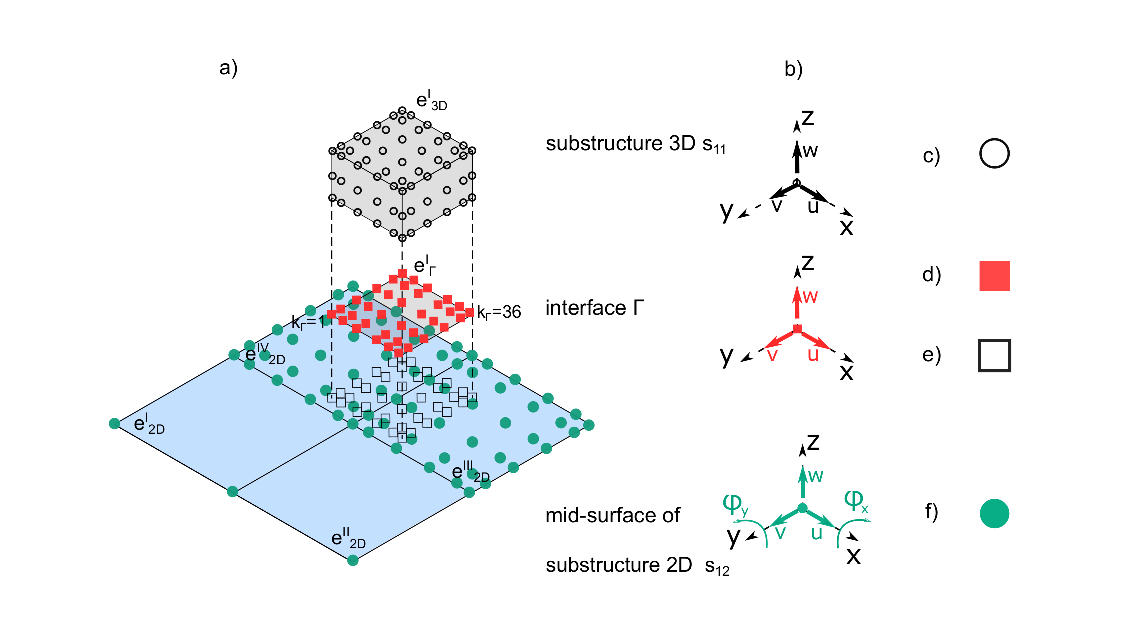
\includegraphics[width=1\textwidth]{Chapter_4/interface_2D3D}
	\end{center}
	\caption{Non-matching interface setup: (\textbf{a}) interface coupling, (\textbf{b}) the interface and the substructures degrees-of-freedom}
	\label{fig:interface}
\end{figure}
The non-matching interface between \ac{2d} and \ac{3d} elements is presented in Figure~\ref{fig:interface}.
The coupling of two domains imposes zero displacements relative to each other.
It can be expressed as
\begin{eqnarray}
	\left\{\begin{array}{c}
		\textbf{u}\\
		\textbf{v}\\
		\textbf{w}
	\end{array}\right\}_{s_{i1}}^{\Gamma^i}-
	\left\{\begin{array}{c}
		\textbf{u}\\
		\textbf{v}\\
		\textbf{w}
	\end{array}\right\}_{s_{i2}}^{\Gamma^i}=
	\left\{\begin{array}{c}
		\textbf{0}\\
		\textbf{0}\\
		\textbf{0}
	\end{array}\right\},
	\label{eq:coupling}
	\nomtypeD[Gamma]{$\Gamma$}{Interface}{}
\end{eqnarray}
where \(s_{i1}\) and \(s_{i2}\) are components connected by the interface \(\Gamma^i\).
For the whole structure, the Eq.~(\ref{eq:coupling}) can be written in the matrix form
\begin{eqnarray}
	\textbf{G}\textbf{d}=\textbf{0},
	\label{eq:cond_disp}
	\nomtypeD[G]{$\textbf{G}$}{Interface coupling matrix}{}
\end{eqnarray}
where \textbf{G} is the coupling matrix which contains the equations to interpolate the substructures displacements at the interfaces, and \(\textbf{d}\) is a global displacement field for \(nS\) number of substructures, composed as
\begin{eqnarray}
	\textbf{d} = \left\{\begin{array}{cccc}
		\textbf{d}_1, & \textbf{d}_2, &\ldots, & \textbf{d}_{nS}
	\end{array}\right\}^T.
	\label{eq:displacements}
\end{eqnarray}

\begin{algorithm}[!tbh]
	\SetAlgoLined
	\For{i = 1 \KwTo 2}{
		create \(n^{\Gamma}\times n^{s_i}\) null matrix 
		\(\mathbf{G}_i\),\\
		\For{j = 1 \KwTo \(n^{\Gamma}\)} {
			find \(ownerElement^j_i\) in the structure \(s_i\)
			containing interface node \(j\) with global coordinates vector: 
			\(X_p=(x^j_p,y^j_p)\)\;
			assign vector \(X_e=(x_e,y_e)\) of coordinates of all nodes in 
			\(ownerElement^j_i\)\;
			assign initial coordinates 
			\(X_{\kappa}=(x^j_{\kappa},y^j_{\kappa})\) to the nearest node in
			\(ownerElement^j_i\) to node \(j\)\;
			transform global coordinates \(X_{\kappa}\) to a local coordinate system \(\xi_{\kappa}=\xi(X_{\kappa}),\  
			\eta_{\kappa}=\eta(X_{\kappa})\)\;
			\While{\(\left|X_p-X_{\kappa}\right|>\mathrm{tol}\)}{
				\(\xi_{\kappa+1}=\xi_{\kappa}+(\mathcal{J}_{\kappa})^{1,1}_{\mathrm{inv}}(x^j_p-x_{\kappa}^j)
				+(\mathcal{J}_{\kappa})^{1,2}_{\mathrm{inv}}(y^j_p-y_{\kappa}^j)\)\,
				\(\eta_{\kappa+1}=\eta_{\kappa}+(\mathcal{J}_{\kappa})^{2,1}_{\mathrm{inv}}(x^j_p-x_{\kappa}^j)
				+(\mathcal{J}_{\kappa})^{2,2}_{\mathrm{inv}}(y^j_p-y_{\kappa}^j)\)\,
				\(X_{\kappa}=N_{\kappa+1}X_e\)\,
			}
			\(\mathbf{G}_i(j,n^{X_e})=N_{\kappa+1}\)\;
		}
		\uIf{\(s_i\) \(\mathrm{is\ 3D}\)} {
			\(\mathbf{G}_i=\left[\begin{array}{ccc}
				\mathbf{G}_i & \mathbf{0} & \mathbf{0}\\
				\mathbf{0} & \mathbf{G}_i & \mathbf{0}\\
				\mathbf{0} & \mathbf{0} & \mathbf{G}_i
			\end{array} \right]
			\)\;
		}
		\ElseIf{\(s_i\) \(\mathrm{is\ 2D}\)} {
			\(\mathbf{G}_i=\left[\begin{array}{ccccc}
				\mathbf{G}_i & \mathbf{0} & \mathbf{0} & 
				\frac{h_i}{2}\mathbf{G}_i & \mathbf{0}\\
				\mathbf{0} & \mathbf{G}_i & \mathbf{0} & \mathbf{0} & 
				\frac{h_i}{2}\mathbf{G}_i\\
				\mathbf{0} & \mathbf{0} & \mathbf{G}_i & \mathbf{0} & 
				\mathbf{0}
			\end{array} \right]\)\;
		}
	}
	\KwResult{coupling matrix \(\mathbf{G}=\left[\begin{array}{cc}
			\mathbf{G}_1 & \mathbf{G}_2
		\end{array} \right]\)}
	where \(s_i\) is one of the coupled structures,\;
	\(n^{\Gamma}\) and \(n^{s_i}\) are node numbers of the interface and node numbers of the structure \(s_i\), respectively \; \(\left(\mathcal{J}_{\kappa}\right)_{\mathrm{inv}}\) is the inverse Jacobian matrix evaluated at \((\xi_{\kappa},\eta_{\kappa})\)\;
	\(N_{\kappa+1}\) is the shape function evaluated at \((\xi_{\kappa+1},\eta_{\kappa+1})\)\;
	\(n^{X_e}\) is the vector of global order numbers of all nodes in the \(ownerElement^j_i\)\;
	\(h_i\) is a thickness of the structure \(s_i\) and tol is a termination criterion for iterations.
	\caption{Interface coupling matrix formulation}
	\label{alg:G_matrix}
	\nomtypeD[Jacobian]{$\mathcal{J}$}{Jacobian matrix}{}%
	\nomtypeD[nmn]{$n,m,n$}{Nodes numbers}{}%
	\nomtypeR[Xp]{$X_p$}{Coordinates vector of the interface point}{}{\unit{\metre}}%
	\nomtypeR[Xe]{$X_e$}{Coordinates vector of the element nodes}{}{\unit{\metre}}%
\end{algorithm}
General formulation of the matrix \textbf{G} is presented in Algorithm \ref{alg:G_matrix}.
The main task in this procedure was to calculate shape functions for each adjacent substructure at the points \(X_p=(x_p^k,y_p^k)\), which are projections of the interface nodes onto these substructures.
The shape function can be calculated after finding an owner element and local coordinates of the points.
Owner element is a spectral element in the domain of the substructure \(s_{ij}\) which contains interface node, for example, interface node \(k_\Gamma=36\) shown in~Figure~\ref{fig:interface}(\textbf{a}) is located in the element \(e^{I}_{3\mathrm{D}}\) and \(e^{III}_{2\mathrm{D}}\) for the substructures \(s_{11}\) and \(s_{12}\), respectively.
It can be found in two ways: using Matlab's built-in function \verb+inpolygon+ or more efficient procedure proposed by Silva et al. \cite{silva2009exact} which was used in the current implementation.
In this procedure, an initial approximation was first performed by rejecting all external points outside the rectangular region bounded by the points \(\mathrm{P_{min}}\) and \(\mathrm{P_{max}}\) as shown in Figure \ref{fig:b_b_test}(\textbf{a}).
If \(\mathrm{X_p}\) is inside the element, then the vectors \(\vec{V}_1\) and \(\vec{V}_2\) have the same direction.
\(\vec{V}_1\) and \(\vec{V}_2\) are defined as
\begin{eqnarray}
	\vec{V}_1 & = & \vec{v}_1\times \vec{v}_p,\\
	\vec{V}_2 & = & \vec{v}_p\times \vec{v}_2.
\label{eq:v_vectors}
\nomtypeD[vvv]{$\vec{v}_p,\,\vec{v}_1,\,\vec{v}_2$}{Cross-product test  vectors}{}%
\nomtypeD[V1]{$\vec{V_1}$}{First cross-product vector}{}%
\nomtypeD[V2]{$\vec{V_2}$}{Second cross-product vector}{}%
\end{eqnarray}
The vectors \(\vec{v}_p\), \(\vec{v_1}\) and \(\vec{v_2}\) are pictured in Figure \ref{fig:b_b_test}(\textbf{b}). \(\vec{V}_1\) and \(\vec{V}_2\) have the same direction if the inequality \(\vec{V}_1 \cdot \vec{V}_2 \geq0\) is satisfied for each element vertex.
Then, the transformation from global to local coordinates was realised by the iterative method presented in the work of Li et al.~\cite{li2014efficient} (see also \verb+while-loop+ in Algorithm~\ref{alg:G_matrix}).
\begin{figure}[!tbh]
	\begin{center}
		\includegraphics[width=0.95\textwidth]{Chapter_4/b_b_test}
	\end{center}
	\caption{Owner element for Xp interface node (\textbf{a}) boundary test, (\textbf{b}) cross-product test}
	\label{fig:b_b_test}
\end{figure}
As the cross product test is applicable only for elements with linear edges, in the case of boundaries approximated by second-order elements, this test was omitted.

The computational effectiveness of Algorithm~\ref{alg:G_matrix} can be easily improved if certain precautions are taken.
Firstly, the mesh of the interface has to be based on the mesh from one of the substructures \(s_{i}\), which may be referred to as a slave.
Shape functions evaluated at (\(\xi\), \(\eta\)) may take only zero and one values.
Moreover, the code was vectorised rather than using a for-loop form, provided that the required matrix of size \(4n^e\times n^{\Gamma}\), where \(n^e\) is the number of elements of the structure \(s_i\) elements, does not exceed the operating memory.
%% SECTION HEADER /////////////////////////////////////////////////////////////////////////////////////
\section{Transformation of the Core Elements}
\label{sec:transformation}

%% SECTION CONTENT ////////////////////////////////////////////////////////////////////////////////////
All core elements are rotated relative to both skins, and thus it is necessary to transform the degrees of freedom from the local coordinate system of the core to the global coordinate system.
For this purpose, an additional sixth \ac{dof} is incorporated, i.e., rotation with respect to the \textit{z}-axis:
\begin{eqnarray}
	\widehat{\textbf{d}}^e_g = \left \{\begin{array}{cccccc}
		\widehat{\textbf{u}}^e & \widehat{\textbf{v}}^e &
		\widehat{\textbf{w}}^e & \widehat{\boldsymbol{\varphi}}_x^e &
		\widehat{\boldsymbol{\varphi}}_y^e & \widehat{\boldsymbol{\varphi}}_z^e
	\end{array}\right \}^T_g.
	\label{eq:d6}
\end{eqnarray}

First, the displacement vector is transformed from the global to local coordinate system by the direction cosines as follows:
\begin{eqnarray}
	\widehat{\textbf{d}}^e_l = \left \{\begin{array}{c}
		\widehat{\textbf{u}}^e \\ \widehat{\textbf{v}}^e \\
		\widehat{\textbf{w}}^e \\ \widehat{\boldsymbol{\varphi}}_x^e \\
		\widehat{\boldsymbol{\varphi}}_y^e
	\end{array}\right \}_l = 
	\left [\begin{array}{ccccc}
		\textbf{V}^e_1, & \textbf{V}^e_2, & \textbf{V}^e_3, & \textbf{0} & \textbf{0} \\
		\textbf{0} & \textbf{0} & \textbf{0} & \textbf{V}^e_1, & \textbf{V}^e_2
	\end{array}\right ]^T
	\left \{\begin{array}{c}
		\widehat{\textbf{u}}^e \\ \widehat{\textbf{v}}^e \\
		\widehat{\textbf{w}}^e \\ \widehat{\boldsymbol{\varphi}}_x^e \\
		\widehat{\boldsymbol{\varphi}}_y^e\\
		\widehat{\boldsymbol{\varphi}}_z^e
	\end{array}\right \}_g,
	\label{eq:d_local}
\end{eqnarray}
where \(\textbf{V}^e_1\),\(\textbf{V}^e_2\) and \(\textbf{V}^e_3\) are direction cosines of the core element. Then, internal forces are calculated according to guideline from Section \ref{sec:gpu} and transformed to a global coordinate system:
\begin{eqnarray}
	\left\{\textbf{F}_{int}\right\}^e_g =
	\left [\begin{array}{ccccc}
		\textbf{V}^e_1, & \textbf{V}^e_2, & \textbf{V}^e_3, & \textbf{0} & \textbf{0} \\
		\textbf{0} & \textbf{0} & \textbf{0} & \textbf{V}^e_1, & \textbf{V}^e_2
	\end{array}\right ]
	\left \{\begin{array}{c}
		\textbf{F}^1_{int} \\
		\textbf{F}^2_{int} \\
		\textbf{F}^3_{int} \\
		\textbf{F}^4_{int} \\
		\textbf{F}^5_{int} \\
	\end{array}\right \}_l^e.
	\label{eq:f_global}
\end{eqnarray}

Additionally, a part of the mass matrix accounted for rotary inertia has to be transformed, and, in contrast to the internal forces vector, this has to be done only once in pre-processing as follows:

\begin{eqnarray}
	\textbf{J}_g=\left [ 
	\begin{array}{ccc}
		\left (\textbf{J}_{11}\right )_g & \left (\textbf{J}_{12}\right )_g & \left (\textbf{J}_{13}\right )_g\\
		& \left (\textbf{J}_{22}\right )_g & \left (\textbf{J}_{23}\right )_g\\
		Sym. &  & \left (\textbf{J}_{33}\right )_g\\
	\end{array}
	\right ]
	=\left[\begin{array}{ccc}
		\textbf{V}_1, \textbf{V}_2, \textbf{V}_3 \end{array}\right ]^T
	\,\textbf{J}_l\,
	\left[\begin{array}{ccc}
		\textbf{V}_1, \textbf{V}_2, \textbf{V}_3 \end{array}\right ].
	\label{eq:inertia}
\end{eqnarray}

As the matrix becomes non-diagonal after transformation, some approximation is necessary.

Surana analysed a lumped mass matrix with non-zero inertia for shell elements \cite{surana1980transition}.
He presented several formulations for a transformed mass matrix to zero off-diagonal values without affecting the results appreciably.
In the presented model, the omission of off-diagonal values of the mass matrix is assumed.
%% SECTION HEADER /////////////////////////////////////////////////////////////////////////////////////
\section{The time integration algorithm}
\label{sec:time}

%% SECTION CONTENT ////////////////////////////////////////////////////////////////////////////////////
The time integration algorithms for the wave propagation can be realised by the step-by-step methods, named Newmark family schemes \cite{newmark1959method}.
The schemes are in general form as
\begin{eqnarray}
	\label{eq:u_newmark}
	\textbf{d}_{t+\Delta t} & = & \textbf{d}_{t} +\Delta t \dot{\textbf{d}}_{t} + \left( 0.5 - \beta \right)\Delta t^2\ddot{\textbf{d}}_{t} + \beta \Delta t^2\ddot{\textbf{d}}_{t+\Delta t},\\
	\dot{\textbf{d}}_{t+\Delta t} & = & \dot{\textbf{d}}_{t} + \Delta t\left(1-\gamma\right)\ddot{\textbf{d}}_{t} + \gamma \Delta t\ddot{\textbf{d}}_{t+\Delta t},
\end{eqnarray}
\nomtypeG[Deltat]{$\Delta t$}{Time increment}{}{\unit{\second}}%
\nomtypeD[betagamma]{$\beta,\,\gamma$}{Time integration parameters}{}%
where \(\Delta t\) is the time increment, \(\textbf{d}_{t}\), and \(\textbf{d}_{t+\Delta t}\) are the displacement vectors in time t, and one step forward, respectively, and \(\beta\) and \(\gamma\) are the integration parameters.
The time discretisation for \(\beta = 0.25\) and \(\gamma = 0.5\), is second-order accurate and the algorithm is a stable, i.e., independent of the time step. It is called an implicit algorithm.
In the case of \(\beta = 0\) and \(\gamma = 0.5\) explicit algorithm is obtain and it is named the central difference method.
In this method for the solution convergence, a time step must be taken much smaller than the Nyquist-Shannon sampling theorem requires.

Considering piezoelectric coupling given by Eq.~(\ref{eq:elecmechcoupling}) and the displacement interface coupling represented by Eq.~(\ref{eq:cond_disp}) the global equation of motion is expressed as
\begin{eqnarray}
	\label{eq:motion_coupling}
	\textbf{M}_{dd}\,\widehat{\ddot{\textbf{d}}} +
	\textbf{D}_{dd}\,\widehat{\dot{\textbf{d}}} +
	\left [\begin{array}{ccc}
		\textbf{K}_{dd}&\textbf{K}_{d\phi}&\textbf{G}^T\\
		\textbf{K}_{d\phi}^T&\textbf{K}_{\phi \phi}&\textbf{0}\\
		\textbf{G}&\textbf{0}&\textbf{0}
	\end{array}\right]
	\left \{\begin{array}{c}
		\widehat{\textbf{d}}\\
		\widehat{\boldsymbol{\phi}}\\
		\widehat{\boldsymbol{\lambda}}
	\end{array}\right\} =
	\left \{\begin{array}{c}
		\widehat{\textbf{f}}_{ext} \\
		\widehat{\textbf{Q}}\\
		\textbf{0}
	\end{array}\right \},
\end{eqnarray}
\nomtypeD[lambda]{$\boldsymbol{\lambda}$}{Lagrange multipliers vector}{}%
where \(\widehat{\boldsymbol{\lambda}}\) is the nodal Lagrange multipliers vector.
Substituting Eq.~(\ref{eq:pztboundary}) and Eq.~(\ref{eq:freePotetial}) into Eq.~(\ref{eq:motion_coupling}), the equation of motion can be rearranged into the form
\begin{eqnarray}
	\textbf{M}_{dd}\,\widehat{\ddot{\textbf{d}}} + \textbf{D}_{dd} \,\widehat{\dot{\textbf{d}}} + (\textbf{K}_{dd}-\textbf{K}_{s}) \,\widehat{\textbf{d}}  = \widehat{\textbf{f}}_{ext} + \widehat{\textbf{f}}_{a} - \textbf{G}^{\mathrm{T}}\,\widehat{\boldsymbol{\lambda}}.
	\label{eq:motionD}
\end{eqnarray}
In the scheme of central difference method, the velocity and acceleration at a certain time \(t\) is given by
\begin{eqnarray}
	\label{eq:v}
	\widehat{\dot{\textbf{d}}}_{t} & = & \frac{\widehat{\textbf{d}}_{t+\Delta t} - \widehat{\textbf{d}}_{t-\Delta t}}{2\Delta t},\\
	\label{eq:a}
	\widehat{\ddot{\textbf{d}}}_{t} & = & \frac{\widehat{\textbf{d}}_{t+\Delta t} - 2\widehat{\textbf{d}}_{t} + \widehat{\textbf{d}}_{t-\Delta t}}{\Delta t^2},
\end{eqnarray}
where \(\widehat{\textbf{d}}_{t-\Delta t}\) is the nodal displacements vector in the previous time step.
Thus, substituting Eq.~(\ref{eq:v}) and (\ref{eq:a}) into Eq.~(\ref{eq:motionD}) and after some rearrangement, global equation of motion can be expressed as
\begin{equation}
	\begin{split}
		\left(\frac{1}{\Delta t^2}\textbf{M}_{dd}+\frac{1}{2\Delta t}\textbf{D}_{dd} \right)\widehat{\textbf{d}}_{t+\Delta t} & = \widehat{\textbf{f}}_{ext} + \widehat{\textbf{f}}_{a} - \left( \textbf{K}_{dd}-\textbf{K}_s\right)\widehat{\textbf{d}}_t
		+ \frac{2}{\Delta t^2}\textbf{M}_{dd}\widehat{\textbf{d}}_t\\
		&-\left(\frac{1}{\Delta t^2}\textbf{M}_{dd}-\frac{1}{2\Delta t}\textbf{D}_{dd}\right)\widehat{\textbf{d}}_{t-\Delta t}-\textbf{G}^{\mathrm{T}}\widehat{\boldsymbol{\lambda}}_t.
	\end{split}
	\label{eq:cdm}
\end{equation}
The most significant advantage of central difference method is that only the sum of the mass and damping matrices needs to be inverted, which is trivial in the presented scheme because both matrices are diagonal.

The vector of Lagrange multipliers \(\widehat{\boldsymbol{\lambda}}_t\) can be extracted from Eq.~(\ref{eq:cdm}) by imposing the constraint (\ref{eq:cond_disp}):
\begin{eqnarray}
	\begin{split}
		\widehat{\boldsymbol{\lambda}}_t & = {\left(\textbf{G}\textbf{L}_+^{-1}\textbf{G}^{\mathrm{T}} 	\right)}^{-1}\textbf{G}\textbf{L}_+^{-1} \Bigg[ \widehat{\textbf{f}}_{ext} + \widehat{\textbf{f}}_{a}\\
		& + \left.\left(\frac{2}{\Delta t^2}\textbf{M}_{dd}-\textbf{K}_{dd}+\textbf{K}_s\right)\widehat{\textbf{d}}_t -\textbf{L}_-\widehat{\textbf{d}}_{t-\Delta t} \right],
	\end{split}
	\label{eq:lambda}
\end{eqnarray}
where \(\textbf{L}_{\pm}=\frac{1}{\Delta t^2}\textbf{M}_{dd}\pm\frac{1}{2\Delta t}\textbf{C}_{dd}\).
The implementation of the central difference method including the excitation and reception of the wave by a pair of \acp{pzt} is presented in Algorithm~\ref{alg:cdm}.

\begin{algorithm}[H]
	\SetAlgoLined
	initialise  \(\widehat{\textbf{d}}_0\), \(\widehat{\dot{\textbf{d}}}_0\), \(\widehat{\boldsymbol{\lambda}}_0\) and \(\boldsymbol{\phi}_{0}\),\\
	calculate \(\widehat{\ddot{\textbf{d}}}_0\) from Eq.~(\ref{eq:motionD}),\\
	select time increment \(\Delta t\leq\Delta t_{cr}\),\\
	extract \(\widehat{\textbf{d}}_{0-\Delta t}\) from Eq. (\ref{eq:v}) and (\ref{eq:a}),\\
	\For{\(\mathrm{each\ time\ step}\)}{
	calculate actuator forces \(\widehat{\textbf{f}}_a\) by Eq.~(\ref{eq:f_act}),\\
	calculate internal forces \(\widehat{\textbf{f}}_{int}=\left(\textbf{K}_{dd}-\textbf{K}_{s}\right)\,\widehat{\textbf{d}}_t\),\\
	calculate Lagrange multipliers \(\widehat{\boldsymbol{\lambda}}\) by Eq.~(\ref{eq:lambda}),\\
	calculate following step displacement \(\widehat{\textbf{d}}_{t+\Delta t}\) solving equation of motion (\ref{eq:cdm}),\\
	calculate sensor response \(\boldsymbol{\phi}_{t+\Delta t}\) by Eq. (\ref{eq:sensorResponse}),\\
	\KwResult{nodal displacement vector \(\widehat\textbf{d}_{t+\Delta t}\) and sensor response \(\boldsymbol{\phi}_{t+\Delta t}\).}
	}
	\caption{Central difference method implementation}
	\label{alg:cdm}
\end{algorithm}

In Eq.~(\ref{eq:lambda}), the matrix \(\left [\textbf{GL}_+^{-1}\textbf{G}^T\right ]\) inversion is necessary to calculate for the each time step.
While \(\textbf{L}_+\) is a diagonal matrix, the sparsity of the matrix \(\textbf{G}\) has a significant effect on the computation cost.
To optimise calculations, the interface mesh should coincide with the mesh from one of the joined structures.
Selected structure is called the \textit{slave} one and the other is the \textit{master}.
In this way, the matrix \(\mathbf{G}_i\) corresponding to slave structure is identity matrix in the case of \ac{3d} elements.
For \ac{2d} elements, \(\mathbf{G}_i\) is block diagonal matrix composed of the identity matrix and the diagonal one with the values of half the thickness of the structure.

%% SECTION HEADER /////////////////////////////////////////////////////////////////////////////////////
\section{Parallel Implementation of the Internal Force Vector Calculation}
\label{sec:gpu}

%% SECTION CONTENT ////////////////////////////////////////////////////////////////////////////////////

The most time-consuming operation in the equation (\ref{eq:motion}) is calculating the internal force vector \(\textbf{f}_{int}=\left(\textbf{K}_{dd}-\textbf{K}_{s}\right)\widehat{\textbf{d}}_{t}\), as the stiffness matrix \(\textbf{K}_{dd}\) occupies a large amount of memory.
Instead of allocating the full matrix \(\textbf{K}_{dd}\), Kudela proposed a parallelized computation of the internal force vector \cite{kudela2016parallel}.
In the pre-processing, the natural derivatives matrix, the vector of inverted components of the Jacobian matrix, and the integration weights multiplied by the Jacobian determinant is rearranged from global to the local form:
\begin{eqnarray}
	\label{eq:isoparametric}
	\textbf{N}^P_{,\xi} & = & \left[ \begin{array}{cccc}
		\textbf{N}^{e=1}_{,\xi} & \textbf{0} & \ldots & \textbf{0}\\
		\textbf{0} & \textbf{N}^{e=2}_{,\xi} & \ldots & \textbf{0}\\
		\vdots & \vdots &  \ddots & \vdots\\
		\textbf{0} & \textbf{0} & \ldots & \textbf{N}^{e=n}_{,\xi}
	\end{array}\right],\\
	\label{eq:jacob}
	\left(\textbf{J}^P\right)^{ij}_{inv} & = & \left\{ \begin{array}{c}
		\left(\textbf{J}^{e=1}\right)^{ij}_{inv}\\
		\left(\textbf{J}^{e=2}\right)^{ij}_{inv}\\
		\vdots\\
		\left(\textbf{J}^{e=n}\right)^{ij}_{inv} \end{array}\right\},\\
	\label{eq:intWeights}
	\textbf{w}^P & = & \left\{ \begin{array}{c}
		\textbf{w}^{e=1}\\
		\textbf{w}^{e=2}\\
		\vdots\\
		\textbf{w}^{e=n} \end{array}\right\} \circ
	\left\{ \begin{array}{c}
		det(\textbf{J})^{e=1}\\
		det(\textbf{J})^{e=2}\\
		\vdots\\
		det(\textbf{J})^{e=n} \end{array}\right\},
\end{eqnarray}
where $n$ is the spectral elements number in modeled domain; \textbf{J} is the Jacobian matrix; $i,j=1\ldots3$; and $\circ$ denotes element-wise multiplication.
The $\textbf{N}^P_{,\xi}$ is a block-diagonal sparse matrix, and the equality of $\textbf{N}^1_{,\xi}=\textbf{N}^2_{,\xi}=\ldots=\textbf{N}^n_{,\xi}$ holds if the same order of interpolation shape function is used for the all elements.
Besides, a vector of local node indices $\textbf{I}_L$ and corresponding global node indices $\textbf{I}_G$ must be defined in the preprocessing process.

Adjacent elements in the mesh share nodes, so one node in the global system can correspond to several nodes in the local system. Since independent operations on vectors are necessary for parallel computation on \ac{gpu}, $I_{G}$ must be rearranged to separate all duplicated nodes. Therefore, the matrix $I_{G}$ is created in which no column has repeated indices of the nodes. Then, the corresponding local map $I_{L}$ must also be created. For the rearrangement algorithm presented in \cite{kudela2016parallel} was used.

The following computational operations are performed during the time integration algorithm. Firstly, the global vector of nodal displacements is transferred to the element nodes displacements such as:

\begin{eqnarray}
	\widehat{\textbf{d}}_t^P = \left\{ \begin{array}{c}
		\widehat{\textbf{d}}_t^{e=1}\\
		\widehat{\textbf{d}}_t^{e=2}\\
		\vdots\\
		\widehat{\textbf{d}}_t^{e=n} \end{array}\right\}.
\end{eqnarray}
Next, the strain and stress vectors are calculated as:
\begin{eqnarray}
	\label{eq:strain}
	\boldsymbol{\epsilon}=\left[\boldsymbol{\epsilon}_{xx},\ \boldsymbol{\epsilon}_{yy},\ \boldsymbol{\epsilon}_{zz},\ \boldsymbol{\gamma}_{yz},\ \boldsymbol{\gamma}_{xz},\ \boldsymbol{\gamma}_{xy}\ \right]^T&=&\textbf{B}^e\widehat{\textbf{d}}^e,\\
	\label{eq:stress}
	\boldsymbol{\sigma}=\left[\boldsymbol{\sigma}_{xx},\ \boldsymbol{\sigma}_{yy},\ \boldsymbol{\sigma}_{zz},\ \boldsymbol{\tau}_{yz},\ \boldsymbol{\tau}_{xz},\ \boldsymbol{\tau}_{xy},\ \right]^T&=&\textbf{C}\boldsymbol{\epsilon}.
\end{eqnarray}
The formulation of equation~\ref{eq:strain} and equation~\ref{eq:stress} for 3D and first-order shear deformation model can be found in \cite{kudela2016parallel} and \cite{kudela2020parallel}, respectively.
Then, the internal forces vector is calculated as:
\begin{eqnarray}
	\label{eq:forces}
	\textbf{F}^P_{int}=\left[\textbf{F}^P_1,\ \textbf{F}^P_2,\ \ldots\ \textbf{F}^P_{n} \right]^T={\textbf{B}^e}^T\boldsymbol{\sigma},
\end{eqnarray}
where $n$ is the nodal degree of freedom.
It should be mentioned that \(\boldsymbol{\epsilon}\), \(\boldsymbol{\sigma}\) and \(\textbf{F}^P_{int}\) components are calculated separately, with the appropriate order of performing the element-wise multiplication of the particular vectors.
This approach is essential in order to keep the calculations matrix-free.

Finally, the assembly of internal forces vector is performed using the \(\textbf{I}_G\) and \(\textbf{I}_L\) as follows:

\begin{eqnarray}
	\label{eq:Fint}
	{\left(\textbf{F}_{int}\right)}^t_{\textbf{I}^m_G} = {\left(\textbf{F}_{int}\right)}^t_{\textbf{I}^m_G} + {\left(\textbf{F}^P_{int}\right)}^t_{\textbf{I}^m_L},\quad for\ m=1\ldots col 
\end{eqnarray}
where \(col\) is the column number of \(\textbf{I}_G\).

In the dissertation, some improvements have been implemented to the above algorithm to make it more computationally efficient.
Instead of calculating the internal forces vector in the for loop like in equation~(\ref{eq:Fint}), it is recommended to assign all local forces into the matrix as:
\begin{eqnarray}
	\label{eq:Fmatrix}
	{\left(\textbf{F}_{int}\right)}^i_{\textbf{I}_G} ={\left(\textbf{F}^P_{int}\right)}^i_{\textbf{I}_L}
\end{eqnarray}
and then return the column vector containing the sum of each row of matrix \({\left(\textbf{F}^P_{int}\right)}^i_{\textbf{I}_L}\).
For example in Matlab, it can be done by built-in function \verb|sum| as:
\begin{eqnarray}
	\label{eq:Fsum}
	{\left(\textbf{F}_{int}\right)}^i = \verb|sum| \left({\left(\textbf{F}^P_{int}\right)}^i_{\textbf{I}_L},2\right);
\end{eqnarray}
Fixed number of columns in equation~(\ref{eq:Fint}) was proposed in \cite{kudela2016parallel}. In the current approach the number of columns is chosen adaptively according to the given mesh. It should be chosen as the smallest divisor of the number of nodes in an element but not less than the maximum number of common elements for a node. In this way, less serial operations are performed and \ac{gpu} resources are better utilized.

Further code modifications included storage scheme. Instead of storing in memory both isoparametric derivatives equation~(\ref{eq:isoparametric}) and inverted components of Jacobian matrix shown in equation~(\ref{eq:jacob}), it is recommended to calculate derivatives in global coordinates system as:
\begin{eqnarray}
	\textbf{N}^P_{,X} = \textbf{J}^{-1}\,\textbf{N}^P_{\xi} 
\end{eqnarray}
Also, a multiplication of elastic constants \(\textbf{C}\) with integration weights defined in equation (\ref{eq:intWeights}) can be performed in preprocessing stage before main loop through integration time steps.

\section{Efficiency of the time integration algorithm}

Two types of simulations were conducted to determine the efficiency of the \ac{pa} to solve the equation of motion shown in Section \ref{sec:gpu}.
The first type compares the \ac{pa} computations performed on the \ac{gpu} and \ac{cpu}.
The second type compares \ac{pa} with the benchmark proposed by Kudela et al.~\cite{kudela2020parallel} named \ac{ba}.
Both analyses were performed on the same workstation as the \ac{ba} equipped with the following components:
\begin{itemize}
	\item \ac{cpu} - Intel Xeon Silver, 2.1 \unit{\giga\Hz}, 8 cores
	\item \ac{gpu} - NVIDIA Tesla V100 32 \unit{\giga\byte} 5120 CUDA cores
	\item RAM - 128 \unit{\giga\byte} DDR4 2933 \unit{\mega\Hz}
\end{itemize}

The comparison \ac{gpu} vs. \ac{cpu} was conducted on a \ac{3d} model of an  aluminium plate (\numproduct{250 x250 x 5} \unit{\cubic\mm}).
The structure was discretised with rectangular mesh of the various number of the in-plane elements.
In each case, a spectral element of \numproduct{6 x 6 x 3} nodes with three \acp{dof} per node was used, with one element through the plate thickness.
The global \ac{dof} and the memory usage are presented in Table~\ref{tab:gpuvscpu}.
A concentrated force was applied to the centre of the plate as a 3-cycle Hann windowed sine at 50 \unit{\kHz} frequency.
\begin{table}[!hbt]
	\tabcolsep=0.2cm
	\centering
	\caption{\label{tab:gpuvscpu} Model parameters used in simulations to compare the algorithm performance on \ac{gpu} and \ac{cpu}.}
	\begin{tabular}{lccccc}
		\toprule
		Number of elements & \numproduct{25 x 25} & \numproduct{50 x 50} & \numproduct{100 x 100} & \numproduct{125 x 125} & \numproduct{250 x 250} \\
		Global \ac{dof}\(\times10^6\) &0.14&0.57&2.26&3.53&14.08\\
		Memory usage \unit{\mega\byte} & 75 & 367 & 1437 & 2252 & 8999\\ \bottomrule
	\end{tabular}
\end{table}
The computational speed up as a function of global \ac{dof} was determined as follows:
\begin{eqnarray}
	\mathrm{Speedup} = \frac{\mathrm{CPU_{avg}}}{\mathrm{GPU_{avg}}},
\end{eqnarray}
where \(\mathrm{CPU_{avg}}\) and \(\mathrm{GPU_{avg}}\) is average one time step calculation performed on \ac{cpu} and \ac{gpu}, respectively.
The time of the pre-/post-processing is not included into the speedup calculation, because the data from \ac{cpu} to \ac{gpu} and vice versa is done only once, while the time integration steps are a large number. 

For the second test computations run times of the simulations conducted on \ac{gpu} were computed for various sizes of the composite plate.
The benchmark parameters proposed in the paper mentioned above are gathered in Table~\ref{tab:benchmark}.
The efficiency of the \ac{pa} regarding \ac{ba} is measured by speedup, defined as the ratio of \ac{ba} run time to \ac{pa}.
\begin{table}[!hbt]
	\tabcolsep=0.2cm
	\centering
	\caption{\label{tab:benchmark}Sample parameters used in the benchmark of the \ac{pa} and the \ac{ba}.}
	\begin{tabular}{lcccccc}
		\toprule
		Plate size \unit{\cm} & \numproduct{30 x 30} & \numproduct{40 x 40} & \numproduct{50 x 50} & \numproduct{70 x 70} & \numproduct{90 x 90} & \numproduct{100 x 100}\\
		Global \ac{dof}\(\times10^6\)&1.02&1.46&1.98&3.09&5.23&6.36\\ \bottomrule
	\end{tabular}
\end{table}

The results of both analysis are pictured in Fig.~\ref{fig:speedup}.
At maximum \ac{dof}, the speedup in \ac{gpu} computation relative to \ac{cpu} computation increases near to 90 and the \ac{pa} is up to ten times more efficient than the \ac{ba}.
Improvement of the algorithm comes from: more operations performed in the pre-processing, transfer of internal forces from the local to the global system by summing columns instead of \verb+for-loop+, and minimized number of columns in the map of local nodes $\textbf{I}_L$ (see section~\ref{sec:gpu}).
\begin{figure}[!tbh]
	\begin{center}
		\includegraphics[width=0.95\textwidth]{Chapter_4/benchmark}
	\end{center}
	\caption{Speedup in function of global \acfp{dof} of the \acf{pa} computation run on \acf{cpu}~vs.~\acf{gpu} (orange dashed line), and compared to \acf{ba} (blue solid line)}
	\label{fig:speedup}
\end{figure}
\section{Conclusions}
\label{sec:conclusionsSEM}
%% SECTION CONTENT ////////////////////////////////////////////////////////////////////////////////////
The Chapter describes the \ac{sem} implementation for use in \acp{hsc} with the \ac{fcgm}.
This model requires the development of structural matrices for \ac{2d} and \ac{3d} elements and a transformation of the nodal displacements between the local and global coordinate systems.
An original approach was developed to connect elements with non-matching grids using an interface based on Lagrange multipliers.
For this purpose, the shape fusions of common points in the space of connected elements were determined to calculate the traction forces necessary to provide joint displacements.

The implementation of the non-matching interface is a major contribution to the development of the \ac{sem} method.
Previously, to connect domains of different shapes, their meshes were matched with each other to enable the connection of nodes.
Without the interface, connecting the specimen components, i.e. the honeycomb core, the rectangular skin and the circular sensor, would have been extremely difficult.
It would probably require assuming some constraints, such as the sensor being located only within the area of the core cell.
The application of the interface goes beyond the dissertation subject; among other things, it was used in the simulation of \ac{gw} registration by the \ac{fbg} optical sensors.

In addition, a parallel central difference method implementation was improved for even more efficient computation on the graphics card.
The obtained equation of motion solution was even 10 times faster than the algorithm presented in the paper \cite{kudela2020parallel}.


% Note that the text in the [] brackets is the one that will
% appear in the table of contents, whilst the text in the {}
% brackets will appear in the main thesis.

%% CHAPTER HEADER /////////////////////////////////////////////////////////////////////////////////////
\chapter[Numerical simulation of the GW in the \ac{hsc}]{Numerical simulation of the GW in the \ac{hsc}}
\label{ch:simulation}

%% CHAPTER INTRODUCTION ///////////////////////////////////////////////////////////////////////////////
This chapter presents the sample configuration for numerical simulations based on the \ac{sem}.
The configuration is consistent with the specimen held for experimental validation of the model.
The description includes the overall dimensions of the \ac{hsc} panel, sensor placement, the materials properties, and the excitation signal.
It is shown how the individual components were meshed to optimise computer operations.
In the chapter, two disbonds models are presented; in the first model, the core cells were removed from the damaged area, and in the second model, the interface elements were removed.
%% INCLUDE SECTIONS ///////////////////////////////////////////////////////////////////////////////////

%% SECTION HEADER /////////////////////////////////////////////////////////////////////////////////////
\section{Sample configuration}
\label{sec:sample}

%% SECTION CONTENT ////////////////////////////////////////////////////////////////////////////////////
The sample of interest was a \numproduct{500 x 500 x 1.5} \unit{\cubic\mm} unidirectional \ac{cfrp} plate with stack sequence \(\left[\ang{0},\,\ang{90}\right]_s\) bonded to an aluminium honeycomb core. The volume fraction of fibres was assumed 47\%.
It was decided to use only one skin, as it is pictured in Fig.~\ref{fig:honeycomb}(b), with the intention of experimental validation and to be able to enlarge disbonds between the skin and the core located in the middle of the \ac{hsc} with a tool in a real sample. 
It was not decided to dedicate separate samples for each size of damage because too many factors would affect the signal value, including skin and sensors properties, the thickness of the adhesive layers, position of the core relative to the sensors, and distance between sensor.
Moreover, it renders closely the realistic scenario of monitoring the same structure.
\begin{figure}[H]
	\begin{center}
		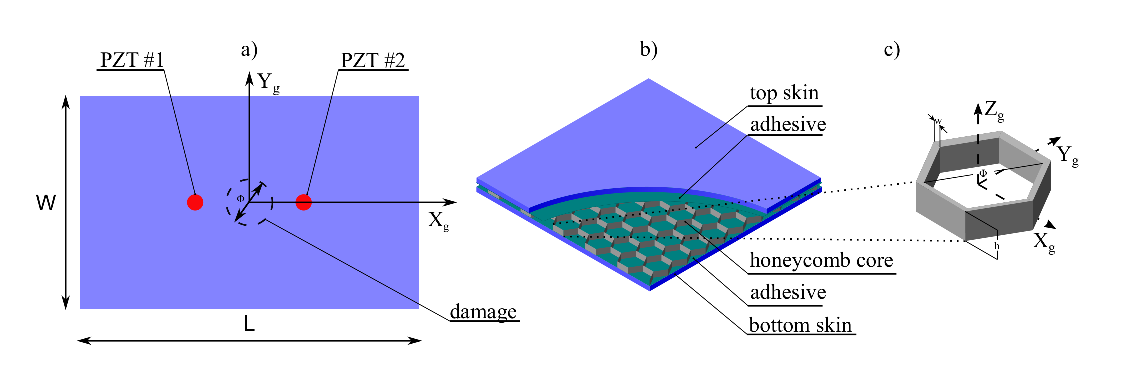
\includegraphics[width=0.95\textwidth]{Chapter_5/honeycomb}
	\end{center}
	\caption{Sample configuration: (\textbf{a}) top view of the sample, (\textbf{b}) \acf{hsc} and (\textbf{c}) details of the honeycomb cell.}
	\label{fig:honeycomb}
\end{figure}

The core geometry is accurately reproduced from the actual specimen, i.e., geometry of irregular hexagonal cells \(\left(\mathrm{h}_1 \ne \mathrm{l}_1\right)\) and double walls at the sheet joints, resulting from the core fabrication technology.
According to the drawing in Fig.~\ref{fig:honeycomb}(\textbf{c}), the cell dimensions are \(\mathrm{w}_c\)=0.1 \unit{\mm}, h\(_1\)=11 \unit{\mm}, h\(_2\)=5 \unit{\mm}, l\(_1\)=10.4 \unit{\mm}, l\(_2\)=6 \unit{\mm} and the cell height g=14.5 \unit{\mm}.
The core was bonded to one \ac{cfrp} plate using the epoxy adhesive (Loctite EA3479B) with the thickness h\(_a\)=0.3 \unit{\mm}.
The adhesive layer covered the entire bottom surface of the skin.

Signal excitation and recording were accomplished with a pair of \acp{pzt}  (Noliac, NCE51) mounted to the top surface of the skin with cyanoacrylate glue.
The circular transducers of diameter \(\Phi_{PZT}\)=10 \unit{\mm} and thickness h\(_{PZT}\)=0.5 \unit{\mm} were attached 200 \unit{\mm} apart, as shown in Fig.~\ref{fig:honeycomb}(\textbf{a}).
The thickness of cyanoacrylate glue under \ac{pzt} was assumed to be h\(_g=50\) \unit{\micro\m}.

The material properties of the components assumed for the simulations are compiled in Tab.~\ref{tab:properties}.
The effective properties of the \ac{cfrp} skin were determined according to the rule of mixtures presented in the book by Vinson and Sierakowski \cite{vinson1993behavior}.
The authors provide a complete description of the homogenisation of composite properties.
Firstly, the stiffness matrix is determined for the single ply of the laminate along the fibre direction.
Then, the stiffness matrix is transformed for other orientations of the laminate plies by the transformation matrix composed of the direction cosines.
In the sample analysed, there are the plies with an orientation of \ang{0} and \ang{90}.
Finally, all the plies in the laminate are homogenised through the thickness.
Explicit expressions of the stiffness components for the laminate modelled by solid elements are presented by Sun and Li in \cite{sun1988three}.
The comprehensive equations to derive the effective stiffness matrix are given in App.~\ref{app:eff_properties} and the resulting \ac{cfrp} properties are shown in Tab.~\ref{tab:properties_eff}.
\begin{table}[H]
	\centering
	\small
	\tabcolsep=0.25cm
	\caption{\label{tab:properties_eff} The effective mechanical properties of the \ac{cfrp} plate and the aluminium honeycomb core for +20\unit{\degreeCelsius}.}
	\begin{tabular}{ccccccccc}
		\toprule
		\multirow{2}{*}{\textbf{Material}} & \(\boldsymbol{E_{11}}\) & \(\boldsymbol{E_{22}}\) & \(\boldsymbol{E_{33}}\) & \(\boldsymbol{G_{12}}\) & \(\boldsymbol{G_{23}}\) & \(\boldsymbol{\nu_{12}}\)	& \(\boldsymbol{\nu_{23}}\) & \(\boldsymbol{\rho}\) \\
		& \unit{\giga\pascal} & \unit{\giga\pascal} & \unit{\giga\pascal} & \unit{\giga\pascal} & \unit{\giga\pascal} & -- & -- & \unit[per-mode = symbol]
		{\kilogram\per\cubic\metre}\\
		\midrule
		\ac{cfrp} & 69.5 & 69.5 & 8.16 & 3.43 & 2.96 & 0.03 & 0.37 & 1555\\
		laminate & & & & & & & &\\
		\midrule
		aluminium & 0.007 & 0.005 & 2.76 & 0.002 & 0.86 & 0.999 & \(\approx0\) & 112\\
		honeycomb & & & & & & & &\\
		\bottomrule
	\end{tabular}
\end{table}
%% SECTION HEADER /////////////////////////////////////////////////////////////////////////////////////
\section{Excitation Signal}
\label{sec:excitation}

%% SECTION CONTENT ////////////////////////////////////////////////////////////////////////////////////
A sine function modulated by the Hann window was chosen as the excitation signal, defined as:
\begin{eqnarray}
	V_e(t) = 0.5\left(1-\cos(2\pi f_m(t-1/f_m)\right)\sin(2\pi f_ct),
\end{eqnarray}
where \(f_c\) is the carrier frequency, and \(f_m=f_c/N_c\) is the modulation frequency with \(N_c\) as the number of cycles.
\(N_c\) was assumed to be five, as a compromise between signal length in the time domain and signal width in the frequency domain.
It is because too high \(N_c\) may cause overlapping wave mods, while too low number will cause increasing signal dispersion.
Both issues can cause difficulties in signal processing for damage assessment.
A carrier frequency in the range \(f_c=[50, 100, 150] \) kHz was considered in the simulation.

%% SECTION HEADER /////////////////////////////////////////////////////////////////////////////////////
\section{Mesh generation for the \acl{fcgm}}
\label{sec:honeycomb}

%% SECTION CONTENT ////////////////////////////////////////////////////////////////////////////////////
The modelled structure was composed of the following components: 2D for the core, epoxy adhesive and cyanoacrylate glue and 3D for the \ac{cfrp} plate and the \acp{pzt}.
Figure~\ref{fig:struct_mesh} depicts the spectral element used to model the wall, the skin and the \ac{pzt}.
During the creation of the core mesh, special attention was taken to minimise the number of non-zero values in the matrix \(\textbf{G}\).
\begin{figure}[H]
	\begin{center}
		\includegraphics[width=0.95\textwidth]{Chapter_5/struct_mesh}
	\end{center}
	\caption{The mesh with the nodes distribution, (\textbf{a}) spectral element used for modeling the wall of the core, (\textbf{b}) excerpt of the skin plate and (\textbf{c}) cyanoacrylate glue mesh with the second-order curve at the boundary}
	\label{fig:struct_mesh}
\end{figure}

The core elements were selected for the slave mesh, with one spectral element dedicated to each honeycomb cell wall.
The master meshes of the skin panel and adhesive layer were divided by three rhombic elements into the area under the core cell.
This way, the interface nodes coincided with those on the hexagon edges (red line in Figure~\ref{fig:struct_mesh}(\textbf{b})).
The map of element nodes and their coordinates were generated by custom code developed in Matlab.
The resulting meshes of the core, adhesive layer and skin are shown in Figure \ref{fig:cas_mesh}.

The mesh for the cyanoacrylate adhesive consisted of five elements, with a second-order curve at the structure boundary, as seen in Figure~\ref{fig:struct_mesh}(\textbf{c}).
This structure was connected to the skin with the non-matching interface elements with the adhesive mesh selected as a slave one.
The \ac{pzt} mesh coincided with the glue mesh and they are connected with the matching interface elements.

\begin{figure}[H]
	\begin{center}
		\includegraphics[width=0.95\textwidth]{Chapter_5/cfrp_mesh}
	\end{center}
	\caption{The meshes of \acl{hsc} components and the interfaces between them}
	\label{fig:cas_mesh}
\end{figure}

%% SECTION HEADER /////////////////////////////////////////////////////////////////////////////////////
\section{GW Propagation in the Homogenized Core Model}
\label{sec:homogenized}

%% SECTION CONTENT ////////////////////////////////////////////////////////////////////////////////////
In dissertation, comparative studies were conducted between the current model and the homogenized one. 
In the simplified model, the values of the material constants of the panel core were calculated according to the method presented by Malek and Gibson \cite{malek2015effective}.
The effective mechanical properties for an aluminium core are gathered in Table \ref{tab:properties_eff}, while the properties for other structures, i.e., the skin, the epoxy adhesive, the cyanoacrylate glue, and the sensors remained unchanged.
The core element has \(6 \times 6 \times 4\) nodes, and the mesh coincides with the skin mesh.
The elements of the other structures are the same as described in the previous section.
%% SECTION HEADER /////////////////////////////////////////////////////////////////////////////////////
\section{GW Propagation in the Damaged Structure}
\label{sec:disbond}

%% SECTION CONTENT ////////////////////////////////////////////////////////////////////////////////////
As the cells in the damaged area become distorted during core separation Figure~\ref{fig:disbond}(\textbf{a}), %PF: label acc. to figure caption.
the damage was modeled by removing the core elements in the disbond area as shown in Figure~\ref{fig:disbond}(\textbf{b}).
\begin{figure}[H]
	%	\begin{center}
	\includegraphics[width=1\linewidth]{Chapter_5/disbond_03}
	%	\end{center}
	\caption{The damaged area in the: (\textbf{a}) experimental sample and (\textbf{b}) numerical mesh.}
	\label{fig:disbond}
\end{figure}
%% SECTION HEADER /////////////////////////////////////////////////////////////////////////////////////
\section{Conclusions}
\label{sec:conclusionsSimul}

%% SECTION CONTENT ////////////////////////////////////////////////////////////////////////////////////
This chapter presents the model configuration that is considered in the dissertation.
The mesh design for each component, the forcing signal, and the damage model are included.
Besides, a homogenisation model is presented for comparison with the proposed model.

% Note that the text in the [] brackets is the one that will
% appear in the table of contents, whilst the text in the {}
% brackets will appear in the main thesis.

%% CHAPTER HEADER /////////////////////////////////////////////////////////////////////////////////////
\chapter[Simulations Results and Model Validation]{Simulations Results and Model Validation}
\label{ch:validation}

%% CHAPTER INTRODUCTION ///////////////////////////////////////////////////////////////////////////////


%% INCLUDE SECTIONS ///////////////////////////////////////////////////////////////////////////////////

%% SECTION HEADER /////////////////////////////////////////////////////////////////////////////////////
\section{Analytical validation of the \ac{pzt} model}
\label{sec:pztVal}

%% SECTION CONTENT ////////////////////////////////////////////////////////////////////////////////////
The current model, i.e. the boundary geometry modelled with the second order elements, is validated by comparing the transducer impedance obtained by numerical simulation and analytical model derived by Giurgiutiu \cite{giurgiutiu2009micromechatronics}.
The impedance Z is a ratio between voltage \((\Phi)\) and current \((I)\) defined as follows:
\begin{eqnarray}
	Z = \frac{\Phi}{I} = \frac{\Phi}{i\omega Q},
\end{eqnarray}
where \(i=\sqrt{-1}\), \(\omega\) is the angular frequency.
In the case of numerical simulation, \(\Phi\) is assumed as the 1.5-cycle Hann windowed sine pulse, and \(Q\) is the charge induced on the electrode calculated by Equation \ref{eq:pzt_sem}. 
The excitation signal has significant values in the 0-300 kHz frequency range, as shown in Fig.~\ref{fig:impedance}(\textbf{a}).
The analytical model is defined as:
\begin{eqnarray}
	Z = \frac{1}{i\omega C_0}\left[\left(1-k_p^2\right)+k_p^2\frac{u_r}{u_I}\right],
\end{eqnarray}
where \(C_0\) is the free capacitance of the sensor, \(k_p\) is the planar coupling coefficient, \(u_r\) is the displacement response, and \(u_I\) is the induced displacement.
Additional, for the comparison, the response of the \ac{sem} with boundary approximation by linear elements was included. 
\begin{figure}[H]
	\begin{center}
		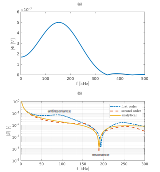
\includegraphics{Chapter_6/impedance}
	\end{center}
	\caption{Validation of the \ac{pzt} model (\textbf{a}) the frequency spectrum of the excitation signal, (\textbf{b}) impedance response of the transducer.}
	\label{fig:impedance}
\end{figure}

It can be notice in Fig.~\ref{fig:impedance}(\textbf{b}) the impedance of the current model is in very good agreement with the analytical solution.
The resonant peak occurred near 190 kHz in both cases, while the resonance of the first-order elements model is shifted 12 kHz toward the higher frequency.
In addition, an antiresonance peak occurred around 90 kHz, not observed in the previous two models.

%% SECTION HEADER /////////////////////////////////////////////////////////////////////////////////////
\section{Experimental setup for the \acs{hsc} model validation}
\label{sec:setup}
%% SECTION CONTENT ////////////////////////////////////////////////////////////////////////////////////
\begin{figure}
	\begin{center}
		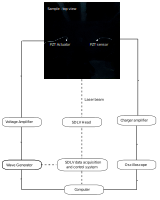
\includegraphics[width=0.95\textwidth]{Chapter_6/setup}
	\end{center}
	\caption{Experimental setup for (1) the \acf{sldv} measurement - dashed line and (2) the \acf{pzt} wave acquisition - solid line.}
	\label{fig:setup}
\end{figure}
The presented model of the \ac{hsc} was validated with results from two experimental studies.
The first one was performed for determination of the full wavefield of the propagating waves by the \ac{sldv} (Polytec PSV–400).
The second study was performed for wave acquisition by the \ac{pzt} sensor.
A schematic of the experimental scenarios is shown in Fig.~\ref{fig:setup}.

The \ac{sldv} is a modern method for non-contact measurement of the vibration velocity of structure surface particles.
The principle of vibrometer operation is based on the Doppler effect, recording the change of frequency of the light beam reflected from the vibrating surface.
In laser vibrometry, the measurement of frequency change is realised by interferometer and analysis of both reference and measurement light beam.
The measuring system is additionally equipped with mirrors allowing to change the angle of the measuring beam, so it is possible to take measurements at a grid of points on a surface of inspected structural element automatically.
The \ac{sldv} setup is presented in Fig.~\ref{fig:sldv}.
\begin{figure}
	\begin{center}
		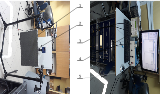
\includegraphics[width=0.95\textwidth]{Chapter_6/sldv}
	\end{center}
	\caption{The \acf{sldv} setup: 1 - the laser sensor head, 2 - the \acf{hsc} specimen, 3 - the arbitrary waveform generator, 4 - the amplifier, 5 - data management system}
	\label{fig:sldv}
\end{figure}

The \ac{pzt} elastic wave generation and acquisition system is used to measure the voltage changes of transducers due to their mechanical deformation.
It is a point measurement at the point of sensor placement.
The following instruments are required to make the measurements: waveform generator to prepare signal, amplifier to strengthen the excitation and recording signals, oscilloscope and central management unit.
The setup used for measurements is shown in Fig.~\ref{fig:pzt_setup}.
\begin{figure}[t]
	\begin{center}
		\includegraphics[width=0.95\textwidth]{Chapter_6/pzt_setup}
	\end{center}
	\caption{The \acf{pzt} setup,(\textbf{a}) elastic wave generation and acquisition instruments:  1 - data management unit - arbitrary wave generator, 2 - oscilloscope - amplifier, 3 , 4 , (\textbf{b}) the specimen held in the environmental chamber.}
	\label{fig:pzt_setup}
\end{figure}

Both methods have some advantages and disadvantages, which are given in the Table~\ref{tab:method_comp}.
\begin{table}[H]
	\small
	\tabcolsep=0.25cm
	%\centering
	\caption{\label{tab:method_comp}Comparison of methods for elastic wave propagation measurements.}
	\begin{tabular}{p{0.1\textwidth}>{\raggedright}p{0.4\textwidth}>{\raggedright \arraybackslash}p{0.4\textwidth}}
		\toprule
		\textbf{Method} &\textbf{Advantages} & \textbf{Disadvantages}\\
		\midrule
		\multirow{5}{*}{\ac{sldv}}   & \tabitem automatic full-field scanning & \tabitem high-cost equipment\\ 
		& \tabitem non-contact measurement & \tabitem long measurement time\\
		& \tabitem \ac{3d} velocity vector (optional)& \tabitem special surface treatment is needed to avoid scattering of the laser beam, e.g. by application of retroreflective tape\\
		& & \tabitem high signal-to-noise ratio\\
		& & \tabitem relatively large space need for measurements \\
		& & \tabitem special sample mounting for repeatability of measurements\\
		\midrule
		\multirow{5}{*}{\ac{pzt}} & \tabitem low-cost instruments & \tabitem spot measurement\\
		& \tabitem high repeatability of measurements & \tabitem displacements vector correlated with the sensor polarization\\
		& \tabitem measurements on the sample in motion & \tabitem cumbersome wiring\\
		& \tabitem generation and recording signals with the same setup & \tabitem sensitive to electric and magnetic fields\\		
		\bottomrule
	\end{tabular}
\end{table}

The sample was fabricated under workshop conditions from the components described in Section~\ref{sec:sample}.
Before applying the two-ingredient glue (Loctite EA3479B), the bottom surface of the skin was cleaned and degreased with the solvent (Loctite SF7063).
The adhesive curing took 48 hours under a distributed load at ambient temperature.

The subject of the parametric study was the effect of the disbond size on the propagating \ac{gw}.
After a reference measurement was made on an intact sample, several measurements were taken for the subsequent damage introduced on the same specimen.
The damage width varied in range \(\mathrm{w_d}=\left [10, 30, 50, 70, 100, 120 \right ]\) \unit{\mm}, while its fixed length was \(\mathrm{l_d} = 175\) \unit{\mm}.

The \(N_c=5\) cycle Hann windowed signal at carrier frequencies \(f_c=[50,100,150]\) \unit{\kHz} was generated using an arbitrary waveform generator (National Instruments, PXI 5413).
The signal was amplified 3.5 times and supplied to the \ac{pzt} actuator (Noliac, NCE51) by the emission/reception unit (LWDS, Cedrat Technologies).
Each measurement was conducted under a temperature of 20\unit{\degreeCelsius} controlled in the environmental chamber (DM 600C, Angelantoni Test Technologies Srl) and averaged 20~times to improve the signal-to-noise ratio.
%% SECTION HEADER /////////////////////////////////////////////////////////////////////////////////////
\section{Results}
\label{sec:resuls}

%% SECTION CONTENT ////////////////////////////////////////////////////////////////////////////////////
The snapshots for the pristine and the damaged sample are shown in \mbox{Figures~\ref{fig:wavefield} and \ref{fig:wavefield_dam5}}, respectively.
One can observe the wave reflections in the core cells for experimental measurements and the present model. 
Additional, the front of the incident wave is distorted for the measurements of 125 and 150 kHz.
The wavefront distortion in the present model is observed in the full range of frequency. 

\vspace{-6pt}
\begin{figure}[H]
	%	\begin{center}
	\includegraphics[width=0.95\linewidth]{Chapter_6/fullfield}
	%	\end{center}
	\caption{The top surface out of plane particle velocity snapshots in time 100 \(\mu\)s for (\textbf{a}) the experimental results obtained by using \ac{sldv}, (\textbf{b}) the present model and (\textbf{c}) the homogenized model in the pristine~sample.}
	\label{fig:wavefield}
\end{figure}
\begin{figure}[H]
	%	\begin{center}
	\includegraphics[width=0.98\linewidth]{Chapter_6/fullfield_dam5}
	%	\end{center}
	\caption{The top surface out of plane particle velocity snapshots in time 100~\(\mu\)s for (\textbf{a}) the experimental results obtained by using \ac{sldv}, (\textbf{b}) the present model and (\textbf{c}) the homogenized model in the sample with 90 mm damage.}
	\label{fig:wavefield_dam5}
\end{figure}

Such  effects are not noticeable in the simplified model because the wave propagates smoothly through the structure.
The wavefront improvement in the experiment and the present model is noticeable in the undamaged region and marked by the red curves in Figure~\ref{fig:wavefield_dam5}.
This is the effect of a lack of reflection with the core.
%% SECTION HEADER /////////////////////////////////////////////////////////////////////////////////////
\section{Conclusions}
\label{sec:conclusionsValid}

%% SECTION CONTENT ////////////////////////////////////////////////////////////////////////////////////

%% CHAPTER HEADER /////////////////////////////////////////////////////////////////////////////////////
\chapter[The Severity of Damage Estimation]{The Severity of Damage Estimation}
\label{ch:severity}

%% CHAPTER INTRODUCTION ///////////////////////////////////////////////////////////////////////////////
A series of computer simulations were performed for different bond sizes for both the \ac{fcgm} and the \ac{hcgm}.
Two damage models were considered, i.e., the removed core cells  and no coupling between the core and the adhesive layer.
The electrical voltage signal captured at the sensor electrode was then analyzed to determine the \ac{madif}.
Several \acfp{di} were used to determine the effect of damage on the propagation waveform.
Of all the indices, those that are monotonic in the assumed damage size range and with the most significant change in index value will be selected for determining the \ac{madif}.
Then, the results are compared with the corresponding indices obtained for experimental measurements.
Lastly, those with the lowest error are chosen for the \ac{madif}.
%% INCLUDE SECTIONS ///////////////////////////////////////////////////////////////////////////////////

%% SECTION HEADER /////////////////////////////////////////////////////////////////////////////////////
\section{Damage indices}
\label{sec:di}

%% SECTION CONTENT ////////////////////////////////////////////////////////////////////////////////////
In the dissertation, six damage indices, considered to be the most effective \cite{torkamani2014novel, moix2016damage}, are analysed based on the signal envelope in the time-domain registered by the sensor.
All of them are considered in three options: (i) the full-length of the signal, (ii) the first wave packet of the \ac{s0}, (iii) the first wave packet of the \ac{a0}.
The analysis will consider signals at 50, 100 and 150 \unit{\kHz}, with the last frequency excluded for the \ac{a0}, because, as indicated in section~\ref{sec:resuls_pzt}, this mode is masked by reflections of the \ac{s0}.
The wave packets are extracted by windowing the full-length signals with a flattened Gaussian window in the form:
\begin{eqnarray}
	g(t)= \mathrm{exp}\left(-\left(\frac{t-t_0}{w_g}\right) ^{n}\right),
	\label{eq:psi_g}
\end{eqnarray}
\nomtypeD[gt]{\(g(t)\)}{Gaussian window}{}%
where \(t_0\) and \(w_g=0.5N_c/f_c\) are the center point and the half-width of the window, respectively, and  \(n\) determines the slope of the window.
The usage of the window is pictured in Fig.~\ref{fig:windows}.
\begin{figure}[!tbh]
	\begin{center}
		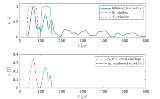
\includegraphics[width=0.95\textwidth]{Chapter_7/windows}
	\end{center}
	\caption{Signal envelop and Gaussian windows}
	\label{fig:windows}
\end{figure}


The following time-domain indices are taken into consideration: \ac{p2p}, \ac{saps}, \ac{sapr}, \acf{rmsd}, \ac{eng} and \ac{cc}.
Definitions of these metrics are given below:

\begin{eqnarray}
	\mathrm{P2P} & = & \left(\mathrm{max}(e_H) - \mathrm{max}(e_D)\right)\\
	\mathrm{SAPS} & = & 1 - \left(\frac{\mathrm{max}(e_H)-\mathrm{max}(e_D)}{\mathrm{max}(e_H)}\right)^2,\\
	\mathrm{SAPR} & = & \frac{\mathrm{max}(e_H)}{\mathrm{max}(e_D)},\\
	\mathrm{RMSD} & = & 1 - \sqrt{\frac{\sum_{i=1}^{n}\left[e_D-e_H\right]^2}	{\sum_{i=1}^{n}e_H^2}},\\
	\mathrm{ENG} & = & 1 -  \frac{\sum_{i=1}^{n}{e_D^2}-\sum_{i=1}^{n}{e_H^2}}{\sum_{i=1}^{n}{e_H^2}},\\
	\mathrm{CC} & = & \frac{n\sum_{i=1}^{n}e_De_H-\sum_{i=1}^{n}e_D\sum_{i=1}^{n}e_H}{\sqrt{n\sum_{i=1}^{n}e_D^2-\left[\sum_{i=1}^{n}e_D\right]^2}\sqrt{n\sum_{i=1}^{n}e_H^2-\left[\sum_{i=1}^{n}e_H\right]^2}},
\end{eqnarray}
where \(e_H\) and \(e_D\) are the envelope of the signal registered by the sensor for the healthy and damaged state of the sample, respectively, and \(n\) is the length of the signal.
The \ac{p2p}, \ac{saps}, \ac{sapr}  are based on the difference between amplitudes of the monitored and the baseline state.
The \ac{rmsd} measures the error between baseline and damaged, \ac{eng} compares the difference of the sensor responses energy and \ac{cc} is the index based on Pearson correlation coefficient.

\begin{figure}[!tbh]
	\begin{center}
		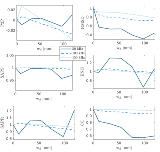
\includegraphics[width=0.95\textwidth]{Chapter_7/DI_full_full}
	\end{center}
	\caption{The \acfp{di} obtained with the \acf{fcgm} based on full-length signals.}
	\label{fig:DI_full_full}
\end{figure}
\begin{figure}[!tbh]
	\begin{center}
		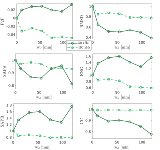
\includegraphics[width=0.95\textwidth]{Chapter_7/DI_full_A0}
	\end{center}
	\caption{The \acfp{di} obtained with the \acf{fcgm} based on \acs{a0} windowed signal.}
	\label{fig:DI_full_A0}
\end{figure}
\begin{figure}[!tbh]
	\begin{center}
		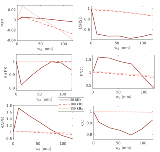
\includegraphics[width=0.95\textwidth]{Chapter_7/DI_full_S0}
	\end{center}
	\caption{The \acfp{di} obtained with the \acf{fcgm} based on \acs{s0} windowed signal.}
	\label{fig:DI_full_S0}
\end{figure}

The \acp{di} based on full-length signals derived from simulations with the \ac{fcgm} are presented in Fig.~\ref{fig:DI_full_full}.
The damage was modelled by removing the core cells in the damage area.
It can be noticed, all the \acp{di} for 50 \unit{\kHz} are not monotonous.
This is due to the fact that a low-frequency wave, according to work of Tian et al. \cite{tian2015wavenumber} up to 100 \unit{\kHz}, propagates through the entire thickness of the \ac{hsc}.
Therefore, in the analysis of damage size, not only the phenomenon of wave leakage is relevant, but also the reflection from cell walls.  
The high-frequency wave propagates mainly through the skin of the panel, so changes in the signal recorded by the sensor in the damaged sample are mainly caused by the wave leakage effect.

The \acp{di} based on the windowed signals are shown in Fig.~\ref{fig:DI_full_A0} and Fig.~\ref{fig:DI_full_S0} for the \ac{a0} and \ac{s0} window, respectively.
It should be mentioned that \acp{di} for 150 \unit{\kHz} are omitted in Fig.~\ref{fig:DI_full_A0}, due to the masking of this mode by the \ac{s0} reflections.
The characteristics of the indices are consistent with the related indices determined for the full-length signals.
However, the values of most windowed signals are lower than those of the full-length signals.
In addition, the \ac{s0} window-based \acp{di} have lower values than the \ac{a0} windowed signals, except the \ac{rmsd} at 50 \unit{kHz}.
It is because dominant displacements of the \ac{s0} are in-plane of the skin, so a smaller portion of the energy of the wave leak into the core through the healthy region.
In the case of the full-length response, the \ac{a0} is registered, which dominant displacements are out of the plate, making this mode more sensitive for damage in the form of disbonds or delamination.

Accordingly, the following indicators are chosen for further consideration: \ac{p2p} and \ac{sapr} at 150 \unit{kHz} (see Fig. \ref{fig:DI_P2P} and Fig. \ref{fig:DI_SAPR}), \ac{rmsd} and \ac{cc}, all in the case of full-length and at 100 and 150 \unit{\kHz} (see Fig. \ref{fig:DI_RMSD_full} and Fig. \ref{fig:DI_CC}), and \ac{rmsd} at 50 \unit{kHz} based on \ac{s0} windowed signals (see Fig. \ref{fig:DI_RMSD_S0}).
Those indices are compered with the \acp{di} obtained with the damage modelled by removing the interface elements and the results from simulations based on the \ac{hcgm} with both damage models.

\begin{figure}[!tbh]
	\begin{center}
		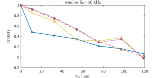
\includegraphics[width=0.95\textwidth]{Chapter_7/DI_P2P}
	\end{center}
	\caption{Comparison of the chosen \acfp{p2p} based on full-length signals for the various models of the core and damage: solid line the \acf{fcgm} with removed core cells, dashed line the \acf{fcgm} with removed interface elements, dash-dot line the \acf{hcgm} with removed core cells, dotted line the \acf{hcgm} with removed interface elements.}
	\label{fig:DI_P2P}
\end{figure}

\begin{figure}[!tbh]
	\begin{center}
		\includegraphics[width=0.95\textwidth]{Chapter_7/DI_SAPR}
	\end{center}
	\caption{Comparison of the chosen \acfp{sapr} based on full-length signals for the various models of the core and damage: solid line the \acf{fcgm} with removed core cells, dashed line the \acf{fcgm} with removed interface elements, dash-dot line the \acf{hcgm} with removed core cells, dotted line the \acf{hcgm} with removed interface elements.}
	\label{fig:DI_SAPR}
\end{figure}
It can be noticed that \ac{p2p} and \ac{sapr} differ significantly in terms of the core model used. Both indexes for the \ac{fcgm} are continuously decreasing, while for the \ac{hcgm}, the values are almost constant in the whole range of damage.
In addition, the damage model has little effect only for the \ac{fcgm}.

\begin{figure}[!tbh]
	\begin{center}
		\includegraphics[width=0.95\textwidth]{Chapter_7/DI_RMSD_S0}
	\end{center}
	\caption{Comparison of the chosen \acfp{rmsd} based on \ac{s0} windowed signals for the various models of the core and damage: solid line the \acf{fcgm} with removed core cells, dashed line the \acf{fcgm} with removed interface elements, dash-dot line the \acf{hcgm} with removed core cells, dotted line the \acf{hcgm} with removed interface elements.}
	\label{fig:DI_RMSD_S0}
\end{figure}

The values for all cases are consistent for the \ac{rmsd} based on the \ac{s0} window.
Only the \ac{fcgm} for the two most minor damages deviates from the other models.
\begin{figure}[!tbh]
	\begin{center}
		\includegraphics[width=0.95\textwidth]{Chapter_7/DI_RMSD_full}
	\end{center}
	\caption{Comparison of the chosen \acfp{rmsd} based on full-length signals for the various models of the core and damage: solid line the \acf{fcgm} with removed core cells, dashed line the \acf{fcgm} with removed interface elements, dash-dot line the \acf{hcgm} with removed core cells, dotted line the \acf{hcgm} with removed interface elements.}
	\label{fig:DI_RMSD_full}
\end{figure}

\begin{figure}[!tbh]
	\begin{center}
		\includegraphics[width=0.95\textwidth]{Chapter_7/DI_CC_full}
	\end{center}
	\caption{Comparison of the chosen \acfp{cc} based on full-length signals for the various models of the core and damage: solid line the \acf{fcgm} with removed core cells, dashed line the \acf{fcgm} with removed interface elements, dash-dot line the \acf{hcgm} with removed core cells, dotted line the \acf{hcgm} with removed interface elements.}
	\label{fig:DI_CC}
\end{figure}

For the \ac{rmsd} and \ac{cc} based on full-length signals, the results are comparable for the all models, except the values for the \ac{hcgm} at 100 \unit{kHz} are more significant than the \ac{fcgm}.

%% SECTION HEADER /////////////////////////////////////////////////////////////////////////////////////
\section{Determination of the \acl{madif}}
\label{sec:determination}

%% SECTION CONTENT ////////////////////////////////////////////////////////////////////////////////////
The \ac{madif} was determined based on the function best fitted to indices selected in the previous subsection.
Since the numerically obtained indices took the shape of a non-linear function, several curves were assumed to find the best fit.
These functions were defined in the general form as follows
\begin{eqnarray}
	y_1(x,a_i) & = & \frac{a_1x}{x+a_2}+a_3,
	\label{eq:function_1}\\
	y_2(x,a_i) & = & a_1\sqrt{x} + a_2x+a_3,
	\label{eq:function_2}\\
	y_3(x,a_i) & = & \frac{a_1x}{\sqrt{a_2 + a_3x^2}}+a_4,\label{eq:function_3} 
\end{eqnarray}
where \(a_i\) are the coefficients of the functions.
The coefficients were determined by built-in function of Matlab named \verb+fminsearch+, which searches for the minimum of a problem specified by \(\min\limits_a f(x,a)\), and the function to be optimised was assumed to be \(f(x,a)=\left\|DI_{num} - y(x,a_i)\right\|\), where \(\left\|\cdot\right\|\) means Euclidean norm.
A criterion for evaluating the fit of the curve to simulation results was a mean absolute error defined as follows
\begin{eqnarray}
	\delta^{\mathrm{fit}} = \frac{1}{\mathrm{n^{DI}}}\sum_{i=1}^{\mathrm{n^{DI}}} \left|\frac{\mathrm{DI^i_{num}}-y(w_d^i)}{\mathrm{DI^i_{num}}}\right|\times100\%,
\end{eqnarray}
where \(\mathrm{n^{DI}}\) is the number of index points.
The examples of the results for \ac{rmsd} are presented in Table~\ref{tab:fit_RMSD_full_FCGM} based on the \ac{fcgm} and in Table~\ref{tab:fit_RMSD_full_HCGM} for the \ac{hcgm}.
The empty cells in the tables mean that the function was fitted with an error of more than 20\%.
The \ac{di} was no longer taken into account if the fit function was not established.
Although prepared, the presentation of a similar summary for the remaining cases was omitted for the Chapter's clarity.
Ultimately, the most fitted function was Eq.~(\ref{eq:function_1}) and Eq.~(\ref{eq:function_2}) for the most \acp{di}.
The best fitted functions were selected to determine the \ac{madif}.

\begin{table}[!tbh]
	\small
	\tabcolsep=0.1cm
	\centering
	\caption{\label{tab:fit_RMSD_full_FCGM} The errors of the functions fitted to the \acf{rmsd} based on full-length windowed signals and the \acf{fcgm}}
	\begin{tabular}{ccccccccccccccc}
		\toprule
		\multirow{3}{*}{\rotatebox[origin=c]{90}{Frequency}} & \multicolumn{7}{c}{\ac{fcgm} - core} & \multicolumn{7}{c}{\ac{fcgm} - interface}\\
		& \multirow{2}{*}{\rotatebox[origin=c]{90}{DI\(_{num}\)}} & \multicolumn{2}{c}{Eq.~(\ref{eq:function_1})} & \multicolumn{2}{c}{Eq.~(\ref{eq:function_2})} & \multicolumn{2}{c}{Eq.~(\ref{eq:function_3})} &
		\multirow{2}{*}{\rotatebox[origin=c]{90}{DI\(_{num}\)}} & \multicolumn{2}{c}{Eq.~(\ref{eq:function_1})} & \multicolumn{2}{c}{Eq.~(\ref{eq:function_2})} & \multicolumn{2}{c}{Eq.~(\ref{eq:function_3})}\\
		& & \(y(w_d^i)\)& \(\delta^{\mathrm{fit}}\) & \(y(w_d^i)\) & \(\delta^{\mathrm{fit}}\) & \(y(w_d^i)\) & \(\delta^{\mathrm{fit}}\) & & \(y(w_d^i)\)& \(\delta^{\mathrm{fit}}\) & \(y(w_d^i)\) & \(\delta^{\mathrm{fit}}\) & \(y(w_d^i)\) & \(\delta^{\mathrm{fit}}\)\\
		\midrule
		\multirow{7}{*}{\rotatebox[origin=c]{90}{100 \unit{\kHz}}} & 1.00 & 1.00 & \multirow{7}{*}{\rotatebox[origin=c]{90}{\textcolor{green}{1.50}}} & 1.00 & \multirow{7}{*}{\rotatebox[origin=c]{90}{1.70}} & 1.00 & \multirow{7}{*}{\rotatebox[origin=c]{90}{1.92}} & 1.00 & 1.00 & \multirow{7}{*}{\rotatebox[origin=c]{90}{\textcolor{green}{1.11}}} & 1.00 & \multirow{7}{*}{\rotatebox[origin=c]{90}{1.45}} & 1.00 & \multirow{7}{*}{\rotatebox[origin=c]{90}{1.31}} \\
		& 0.83 & 0.85 & & 0.88 & & 0.84 & & 0.92 & 0.92 & & 0.90 & & 0.94 & \\ 
		& 0.82 & 0.80 & & 0.82 & & 0.79 & & 0.85 & 0.84 & & 0.83 & & 0.85 & \\ 
		& 0.80 & 0.78 & & 0.79 & & 0.78 & & 0.79 & 0.79 & & 0.79 & & 0.80 & \\ 
		& 0.76 & 0.78 & & 0.78 & & 0.78 & & 0.76 & 0.77 & & 0.76 & & 0.77 & \\ 
		& 0.77 & 0.77 & & 0.77 & & 0.78 & & 0.73 & 0.75 & & 0.74 & & 0.76 & \\ 
		& 0.75 & 0.77 & & 0.78 & & 0.78 & & 0.75 & 0.73 & & 0.72 & & 0.75 & \\
		\midrule
		\multirow{7}{*}{\rotatebox[origin=c]{90}{150 \unit{\kHz}}} & 1.00 & 1.00 & \multirow{7}{*}{\rotatebox[origin=c]{90}{3.10}} & 1.00 & \multirow{7}{*}{\rotatebox[origin=c]{90}{\textcolor{green}{1.28}}} & 1.00 & \multirow{7}{*}{\rotatebox[origin=c]{90}{6.83}} & 1.00 & 1.00 & \multirow{7}{*}{\rotatebox[origin=c]{90}{1.32}} & 1.00 & \multirow{7}{*}{\rotatebox[origin=c]{90}{\textcolor{green}{0.73}}} & 1.00 & \multirow{7}{*}{\rotatebox[origin=c]{90}{4.85}} \\
		& 0.89 & 0.95 & & 0.92 & & 0.97 & & 0.93 & 0.96 & & 0.95 & & 0.97 & \\ 
		& 0.85 & 0.87 & & 0.85 & & 0.91 & & 0.89 & 0.89 & & 0.88 & & 0.92 & \\ 
		& 0.80 & 0.81 & & 0.79 & & 0.85 & & 0.83 & 0.83 & & 0.82 & & 0.87 & \\ 
		& 0.74 & 0.76 & & 0.74 & & 0.80 & & 0.76 & 0.77 & & 0.77 & & 0.82 & \\ 
		& 0.68 & 0.71 & & 0.70 & & 0.75 & & 0.71 & 0.72 & & 0.72 & & 0.76 & \\ 
		& 0.64 & 0.67 & & 0.65 & & 0.70 & & 0.67 & 0.68 & & 0.67 & & 0.71 & \\ 
		\bottomrule
	\end{tabular}
\end{table}

\begin{table}[!tbh]
	\small
	\tabcolsep=0.1cm
	\centering
	\caption{\label{tab:fit_RMSD_full_HCGM} The errors of the functions fitted to the \acf{rmsd} based on full-length windowed signals and the \acf{hcgm}}
	\begin{tabular}{ccccccccccccccc}
		\toprule
		\multirow{3}{*}{\rotatebox[origin=c]{90}{Frequency}} & \multicolumn{7}{c}{\ac{hcgm} - core} & \multicolumn{7}{c}{\ac{hcgm} - interface}\\
		& \multirow{2}{*}{\rotatebox[origin=c]{90}{DI\(_{num}\)}} & \multicolumn{2}{c}{Eq.~(\ref{eq:function_1})} & \multicolumn{2}{c}{Eq.~(\ref{eq:function_2})} & \multicolumn{2}{c}{Eq.~(\ref{eq:function_3})} &
		\multirow{2}{*}{\rotatebox[origin=c]{90}{DI\(_{num}\)}} & \multicolumn{2}{c}{Eq.~(\ref{eq:function_1})} & \multicolumn{2}{c}{Eq.~(\ref{eq:function_2})} & \multicolumn{2}{c}{Eq.~(\ref{eq:function_3})}\\
		& & \(y(w_d^i)\)& \(\delta^{\mathrm{fit}}\) & \(y(w_d^i)\) & \(\delta^{\mathrm{fit}}\) & \(y(w_d^i)\) & \(\delta^{\mathrm{fit}}\) & & \(y(w_d^i)\)& \(\delta^{\mathrm{fit}}\) & \(y(w_d^i)\) & \(\delta^{\mathrm{fit}}\) & \(y(w_d^i)\) & \(\delta^{\mathrm{fit}}\)\\
		\midrule
		\multirow{7}{*}{\rotatebox[origin=c]{90}{100 \unit{\kHz}}} & 1.00 & 1.00 & \multirow{7}{*}{\rotatebox[origin=c]{90}{\textcolor{green}{5.37}}} & 1.00 & \multirow{7}{*}{\rotatebox[origin=c]{90}{9.85}} & \multirow{7}{*}{-} & \multirow{7}{*}{-} & 1.00 & 1.00 & \multirow{7}{*}{\rotatebox[origin=c]{90}{7.40}} & 1.00 & \multirow{7}{*}{\rotatebox[origin=c]{90}{\textcolor{green}{6.22}}} & 1.00 & \multirow{7}{*}{\rotatebox[origin=c]{90}{11.15}} \\
		& 0.55 & 0.57 & & 0.71 & & & & 0.67 & 0.75 & & 0.74 & & 0.80 & \\ 
		& 0.57 & 0.53 & & 0.58 & & & & 0.61 & 0.57 & & 0.59 & & 0.58 & \\ 
		& 0.57 & 0.52 & & 0.54 & & & & 0.53 & 0.50 & & 0.51 & & 0.51 & \\ 
		& 0.48 & 0.51 & & 0.52 & & & & 0.45 & 0.46 & & 0.46 & & 0.48 & \\ 
		& 0.50 & 0.51 & & 0.53 & & & & 0.35 & 0.44 & & 0.42 & & 0.47 & \\ 
		& 0.47 & 0.51 & & 0.55 & & & & 0.42 & 0.42 & & 0.40 & & 0.46 & \\ 
		\midrule
		\multirow{7}{*}{\rotatebox[origin=c]{90}{150 \unit{\kHz}}} & 1.00 & 1.00 & \multirow{7}{*}{\rotatebox[origin=c]{90}{0.51}} & 1.00 & \multirow{7}{*}{\rotatebox[origin=c]{90}{\textcolor{green}{0.33}}} & 1.00 & \multirow{7}{*}{\rotatebox[origin=c]{90}{2.41}} & 1.00 & 1.00 & \multirow{7}{*}{\rotatebox[origin=c]{90}{\textcolor{green}{0.79}}} & 1.00 & \multirow{7}{*}{\rotatebox[origin=c]{90}{\textcolor{green}{0.79}}} & \multirow{7}{*}{-} & \multirow{7}{*}{-} \\
		& 0.96 & 0.97 & & 0.97 & & 0.98 & & 0.95 & 0.95 & & 0.94 & & & \\ 
		& 0.93 & 0.93 & & 0.93 & & 0.95 & & 0.88 & 0.89 & & 0.89 & & & \\ 
		& 0.89 & 0.89 & & 0.89 & & 0.91 & & 0.84 & 0.85 & & 0.85 & & & \\ 
		& 0.85 & 0.85 & & 0.85 & & 0.88 & & 0.82 & 0.82 & & 0.82 & & & \\ 
		& 0.81 & 0.81 & & 0.81 & & 0.84 & & 0.80 & 0.79 & & 0.79 & & & \\ 
		& 0.77 & 0.78 & & 0.78 & & 0.80 & & 0.76 & 0.77 & & 0.76 & & & \\ 
		\bottomrule
	\end{tabular}
\end{table}

Then all selected \acp{di} and their fitted functions were compared with experimental results.
The best results were obtained for the \ac{rmsd} and the \ac{cc} based on the full-length signals at 100 \unit{kHz}. 
Those indices are presented in Figures~\ref{fig:madif_rmsd_best} and \ref{fig:madif_cc_best}, respectively.
\begin{figure}[!tbh]
	\begin{center}
		\includegraphics[width=0.95\textwidth]{Chapter_7/MADIF_RMSD_100_best_err}
	\end{center}
	\caption{(\textbf{a}) Comparison of the \acl{madif} based on the \acf{rmsd} and the experimental results, and (\textbf{b}) the percentage error between them}
	\label{fig:madif_rmsd_best}
\end{figure}

\begin{figure}[!tbh]
	\begin{center}
		\includegraphics[width=0.95\textwidth]{Chapter_7/MADIF_CC_100_best_err}
	\end{center}
	\caption{(\textbf{a}) Comparison of the \acf{madif} based on \acf{cc} and the experimental results, and (\textbf{b}) the percentage error between them}
	\label{fig:madif_cc_best}
\end{figure}

Both indices achieved the lowest error around 5\% for the \ac{fcgm}, with the interface elements removed as the damage model.
The indices were also in very good agreement for the \ac{fcgm} with removed cells as a damage model.
In the case of the \ac{hcgm}, unsatisfactory results were obtained, as none of the indices correspond to the experimental ones with an error of less than 20\%.
What may be relevant here is that the wave continuously transmits energy to the core throughout its propagation.
In contrast, in the case of the \ac{fcgm}, the wave transmits energy incidentally, when it encounters the core walls.
\pagebreak

According to the analysis, the \ac{rmsd} and the \ac{cc} based on the \ac{fcgm} and full-length signals at 100 \unit{kHz} were chosen as the \ac{madif}.
From Eq. (\ref{eq:function_1}), they were defined as follows:
\begin{eqnarray}
	MADIF^{RMSD}(w_d) & = & {13.44w_d}/(w_d+38.12)+0.64,
	\label{eq:MADIF_RMSD}\\
	MADIF^{CC}(w_d) & = & 16.62w_d/(w_d+133.05)+0.88.
	\label{eq:MADIF_CC}
\end{eqnarray}

The comparison of the \ac{madif} and the \ac{edif} based on the \ac{rmsd} and the \ac{cc} are presented in Figure~\ref{fig:madif_20}.
The \ac{edif} was found based on experimental measurements, using the fit function from Eq.~(\ref{eq:function_1}) (the same as the \ac{madif}).
The \ac{rmsd} is in excellent agreement with the experimentally obtained index, achieving an absolute error of less than 4 mm over the full range of damage.
The result of the \ac{cc} is less satisfactory, but it also agrees with the experimentally obtained index.
The absolute error is less than 9 mm.
\pagebreak
Both indices can be used to estimate the damage size in the assumed scenario with a proposed approximation function.
\begin{figure}[!tbh]
	\begin{center}
		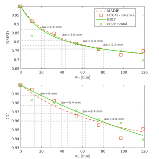
\includegraphics[width=1.0\textwidth]{Chapter_7/MADIF_20}
	\end{center}
	\caption{The \acl{madif} and the \acf{edif} based on the \acf{rmsd} 100 \unit{\kHz}}
	\label{fig:madif_20}
\end{figure}


\section{Conclusions}
\label{sec:conclusionsSever}
In this chapter, the \ac{madif} was determined by which the milestone of the dissertation was achieved.
For this purpose, six \acp{di} were analysed for two different models of the panel core and two models of the damage.

Among the indices, the best two \acp{di} were selected to determine the \ac{madif} function.
Their characteristics are monotonic over the entire damage range and a significant change in the index value for the most extensive damage.
The numerical results are in excellent agreement with the experimental measurements.
The \ac{hcgm} proved inadequate for determining the \ac{madif}, as all tested \acp{di} reached a mean error of more than 20\% relative to the experimental measurements.

The presented analysis demonstrates the confirmation of the thesis that it is possible to determine the damage severity function in \ac{hsc} by employing numerical simulations.
It concerns a rectangular defect between the sensors, so that it can be the basis for further studies with various shapes and positions of damage.
% Note that the text in the [] brackets is the one that will
% appear in the table of contents, whilst the text in the {}
% brackets will appear in the main thesis.

%% CHAPTER HEADER /////////////////////////////////////////////////////////////////////////////////////
\chapter[GW Propagation under Variable Temperature Conditions]{GW Propagation under Variable Temperature Conditions}
\label{ch:tempEffects}

%% CHAPTER INTRODUCTION ///////////////////////////////////////////////////////////////////////////////


%% INCLUDE SECTIONS ///////////////////////////////////////////////////////////////////////////////////

%% SECTION HEADER /////////////////////////////////////////////////////////////////////////////////////
\section{Temperature-Dependent Elastic Properties}
\label{sec:tempProperties}

%% SECTION CONTENT ////////////////////////////////////////////////////////////////////////////////////

%% SECTION HEADER /////////////////////////////////////////////////////////////////////////////////////
\section{Experimental Validation of Temperature Effects on the GW propagation}
\label{sec:tempSetup}

%% SECTION CONTENT ////////////////////////////////////////////////////////////////////////////////////

%% SECTION HEADER /////////////////////////////////////////////////////////////////////////////////////
\section{Results}
\label{sec:tempResults}

%% SECTION CONTENT ////////////////////////////////////////////////////////////////////////////////////

%% SECTION HEADER /////////////////////////////////////////////////////////////////////////////////////
\section{Conclusions}
\label{sec:conclusionsTemp}

%% SECTION CONTENT ////////////////////////////////////////////////////////////////////////////////////

% Note that the text in the [] brackets is the one that will
% appear in the table of contents, whilst the text in the {}
% brackets will appear in the main thesis.

%% CHAPTER HEADER /////////////////////////////////////////////////////////////////////////////////////
\chapter[Summary]{Summary}
\label{ch:summary}

This dissertation develops a model-assisted method for identifying the severity of mechanical damage in a honeycomb sandwich composite. 
For this purpose, the guided wave method was used, based on the change in elastic wave propagation under the influence of their interaction with damage in the monitored structure.
A phenomenon called wave leakage in sandwich panels results in the transmission of the wave into the structure core, where wave energy is attenuated.
In the case of damage such as disbonds of the core from the skin, the phenomenon does not occur.
Thus, a signal recorded by a sensor is distorted regarding a healthy one.

The effect of damage size on wave propagation was done using computer simulations, resulting in a model-assisted identification function.
Due to the high complexity of the structure under analysis, an accurate and efficient model had to be used.
It was achieved by engaging the spectral element method, one of the most robust tools for modelling elastic wave propagation.
Chapter \ref{ch:sem} presents a full implementation of the method for the honeycomb sandwich composite.
One- and two-dimensional spectral elements are used in the model, and a multi-physics model of piezoelectric transducers is implemented for the excitation and recording of guided waves.
This approach required the development of an interface to connect all the elements.
The dissertation presents a new method to determine the non-matching interface elements using the shape function of the spectral elements.

Two core models were analysed, i.e. (i) the full core geometry model and (ii) the homogenised core geometry model.
A rectangular core-skin disbond of variable width and fixed length was taken as the damage placed in the centre of the panel.
The defect was modelled by removing (i) the core cells and (ii) the interface elements.
Then, after the model validation presented in chapter \ref{ch:validation}, computer simulations were performed for different damage sizes and varied excitation signal frequencies.

Obtained signals were proceeded and then used to determine several damage indices.
It turned out that only two indices satisfied the selection criterion, i.e. monotonic over the full range of damage size and the magnitude of the function value.
These two functions are the indices based on root mean square deviation and correlation coefficient for 100 kHz signals and fulfil the criteria for all models.
After comparing model-assisted damage identification functions with the experimental results, it appears that the full core geometry model is more accurate than the homogenised one.
That model with the index based on root mean square deviation achieved an excellent agreement with the experimental investigation.

In Chapter \ref{ch:tempEffects}, an analysis of the effect of ambient temperature on the function is presented.
A parametric study followed this to determine the effect of varied components parameters on the elastic wave propagation in honeycomb sandwich composite. 
It turns out that some parameters only affect the determination of the reference signals, and some depend on the conditions prevailing during the structure inspection.
It is recommended that an effective tool be developed to work out the current parameters of the structure.

Major contribution of the dissertation are:
\begin{itemize}
	\item develop of the full core geometry model based on spectral element method;
	\item develop of the non-matching interface elements,
	\item determination of the model-assisted damage identification function for honeycomb sandwich composite,
	\item time-defendant study on the model-assisted damage identification function
	\item optimisation of the time integration algorithm for parallel computation on graphics processing unit.
\end{itemize}

The dissertation proved the thesis validity: model-assisted analysis of guided wave propagation is an effective tool for determining the damage severity in honeycomb sandwich composites.
The results achieved in the dissertation encourage further work on this topic.
Namely, the analysis of functions for damage with different shapes, e.g. circles or ellipses, different positions.

% Note that the text in the [] brackets is the one that will
% appear in the table of contents, whilst the text in the {}
% brackets will appear in the main thesis.

%% CHAPTER HEADER /////////////////////////////////////////////////////////////////////////////////////

%% CHAPTER INTRODUCTION ///////////////////////////////////////////////////////////////////////////////

\appendix
%% INCLUDE SECTIONS ///////////////////////////////////////////////////////////////////////////////////
% Note that the text in the [] brackets is the one that will
% appear in the table of contents, whilst the text in the {}
% brackets will appear in the main thesis.

%% APPENDIX HEADER ////////////////////////////////////////////////////////////////////////////////////

\chapter{Formulas for calculation of internal forces}
\label{app:fu}

%% APPENDIX CONTENT ///////////////////////////////////////////////////////////////////////////////////
In the pre-processing operations, the product of the stiffness coefficients, integration weighs and Jacobian determinant must be determined:
\begin{eqnarray}
	\mathcal{C}^P_{i,j} &=& \textbf{C}^P_{i,j}\circ\mathcal{W}^P,\,i,j=1,2,3,4,5,6\\
	\mathcal{A}^P_{i,j} &=& \textbf{A}^P_{i,j}\circ\mathcal{W}^P,\,i,j=1,2,6,\\
	\hat{\mathcal{A}}^P_{i,j} &=& \hat{\textbf{A}}^P_{i,j}\circ\mathcal{W}^P,\,i,j=4,5,\\
	\mathcal{B}^P_{i,j} &=& \textbf{B}^P_{i,j}\circ\mathcal{W}^P,\,i,j=1,2,6,\\
	\mathcal{D}^P_{i,j} &=& \textbf{D}^P_{i,j}\circ\mathcal{W}^P\, \mathrm{for}\, i,j=1,2,6,
\end{eqnarray}
and derivatives in global coordinates system:
\begin{eqnarray}
\frac{\partial \textbf{N}^P}{\partial x} &=& \textbf{N}^P_{,\xi}\circ\left(\mathcal{J}^P\right)^{1,1}_{\mathrm{inv}} + \textbf{N}^P_{,\eta}\circ\left(\mathcal{J}^P\right)^{2,1}_{\mathrm{inv}} + \textbf{N}^P_{,\zeta}\circ\left(\mathcal{J}^P\right)^{3,1}_{\mathrm{inv}},\\
\frac{\partial \textbf{N}^P}{\partial y} &=& \textbf{N}^P_{,\xi}\circ\left(\mathcal{J}^P\right)^{1,2}_{\mathrm{inv}} + \textbf{N}^P_{,\eta}\circ\left(\mathcal{J}^P\right)^{2,2}_{\mathrm{inv}} + \textbf{N}^P_{,\zeta}\circ\left(\mathcal{J}^P\right)^{3,2}_{\mathrm{inv}},\\
\frac{\partial \textbf{N}^P}{\partial z} &=& \textbf{N}^P_{,\xi}\circ\left(\mathcal{J}^P\right)^{1,3}_{\mathrm{inv}} + \textbf{N}^P_{,\eta}\circ\left(\mathcal{J}^P\right)^{2,3}_{\mathrm{inv}} + \textbf{N}^P_{,\zeta}\circ\left(\mathcal{J}^P\right)^{3,3}_{\mathrm{inv}}.
\end{eqnarray}

The determination of the internal force field is carried out in four steps for each moment.
In the first step, the displacement vectors are calculated, which in the case of \ac{3d} elements, are defined as:
\begin{eqnarray}
	\label{eq:strain}
	\boldsymbol{\epsilon}^P_{xx} &=& \frac{\partial \textbf{N}^P}{\partial x}\, \widehat{\textbf{u}}^P,\\
	\boldsymbol{\epsilon}^P_{yy} &=& \frac{\partial \textbf{N}^P}{\partial y}\, \widehat{\textbf{v}}^P,\\
	\boldsymbol{\epsilon}^P_{zz} &=& \frac{\partial \textbf{N}^P}{\partial z}\, \widehat{\textbf{w}}^P,\\
	\boldsymbol{\gamma}^P_{yz} &=& \frac{\partial \textbf{N}^P}{\partial y}\, \widehat{\textbf{w}}^P + \frac{\partial \textbf{N}^P}{\partial z}\, \widehat{\textbf{v}}^P,\\
	\boldsymbol{\gamma}^P_{xz} &=&  \frac{\partial \textbf{N}^P}{\partial x}\, \widehat{\textbf{w}}^P + \frac{\partial \textbf{N}^P}{\partial z}\, \widehat{\textbf{u}}^P,\\
	\boldsymbol{\gamma}^P_{xy} &=&  \frac{\partial \textbf{N}^P}{\partial x}\, \widehat{\textbf{v}}^P + \frac{\partial \textbf{N}^P}{\partial y}\, \widehat{\textbf{u}}^P.
\end{eqnarray}
Then the stress vectors are calculated as follows: 
\begin{eqnarray}
	\label{eq:stress}
	\boldsymbol{\sigma}^P_{xx} &=& \mathcal{C}^P_{1,1}\circ\boldsymbol{\epsilon}^P_{xx} +  \mathcal{C}^P_{1,2}\circ\boldsymbol{\epsilon}^P_{yy} + \mathcal{C}^P_{1,3}\circ\boldsymbol{\epsilon}^P_{zz} +
	\mathcal{C}^P_{1,6}\circ\boldsymbol{\gamma}^P_{xy},\\
	\boldsymbol{\sigma}^P_{yy} &=& \mathcal{C}^P_{2,1}\circ\boldsymbol{\epsilon}^P_{xx} +  \mathcal{C}^P_{2,2}\circ\boldsymbol{\epsilon}^P_{yy} + \mathcal{C}^P_{2,3}\circ\boldsymbol{\epsilon}^P_{zz} +
	\mathcal{C}^P_{2,6}\circ\boldsymbol{\gamma}^P_{xy},\\
	\boldsymbol{\sigma}^P_{zz} &=& \mathcal{C}^P_{3,1}\circ\boldsymbol{\epsilon}^P_{xx} +  \mathcal{C}^P_{3,2}\circ\boldsymbol{\epsilon}^P_{yy} + \mathcal{C}^P_{3,3}\circ\boldsymbol{\epsilon}^P_{zz} +
	\mathcal{C}^P_{3,6}\circ\boldsymbol{\gamma}^P_{xy},\\
	\boldsymbol{\tau}^P_{yz} &=& \mathcal{C}^P_{4,4}\circ\boldsymbol{\gamma}^P_{yz} +  \mathcal{C}^P_{4,5}\circ\boldsymbol{\gamma}^P_{xz},\\
	\boldsymbol{\tau}^P_{xz} &=& \mathcal{C}^P_{5,4}\circ\boldsymbol{\gamma}^P_{yz} +  \mathcal{C}^P_{5,5}\circ\boldsymbol{\gamma}^P_{xz},\\
	\boldsymbol{\tau}^P_{xy} &=& \mathcal{C}^P_{1,6}\circ\boldsymbol{\epsilon}^P_{xx} +  \mathcal{C}^P_{2,6}\circ\boldsymbol{\epsilon}^P_{yy} + \mathcal{C}^P_{3,6}\circ\boldsymbol{\epsilon}^P_{zz} +
	\mathcal{C}^P_{6,6}\circ\boldsymbol{\gamma}^P_{xy}.
\end{eqnarray}
The next step is calculation of the effective global forces for each element along x, y and z, directions, respectively.
\begin{eqnarray}
	\label{eq:force_3d}
	\textbf{F}^P_{x} &=& 
	\left( \frac{\partial \textbf{N}^P}{\partial x}\right)^T \boldsymbol{\sigma}^P_{xx} +
	\left( \frac{\partial \textbf{N}^P}{\partial y}\right)^T \boldsymbol{\sigma}^P_{xy} +
	\left( \frac{\partial \textbf{N}^P}{\partial z}\right)^T \boldsymbol{\sigma}^P_{xz},\\
	\textbf{F}^P_{y} &=&  
	\left( \frac{\partial \textbf{N}^P}{\partial x}\right)^T \boldsymbol{\sigma}^P_{xy} +
	\left( \frac{\partial \textbf{N}^P}{\partial y}\right)^T \boldsymbol{\sigma}^P_{yy} +
	\left( \frac{\partial \textbf{N}^P}{\partial z}\right)^T \boldsymbol{\sigma}^P_{yz},\\
	\textbf{F}^P_{z} &=&  
	\left( \frac{\partial \textbf{N}^P}{\partial x}\right)^T \boldsymbol{\sigma}^P_{xz} +
	\left( \frac{\partial \textbf{N}^P}{\partial y}\right)^T \boldsymbol{\sigma}^P_{yz} +
	\left( \frac{\partial \textbf{N}^P}{\partial z}\right)^T \boldsymbol{\sigma}^P_{zz}.
\end{eqnarray}
Finally, the element wise forces vectors are assembly to global vectors according to Eq. (\ref{eq:Fmatrix}) and Eq. (\ref{eq:Fsum}).

Similarly, internal forces are determined for \ac{2d} elements, with displacement vectors defined as:
\begin{eqnarray}
	\label{eq:strain_b}
	\boldsymbol{\epsilon}^P_{b1} &=& \frac{\partial \textbf{N}^P}{\partial x}\, \widehat{\textbf{u}}^P_0,\\
	\boldsymbol{\epsilon}^P_{b2} &=& \frac{\partial \textbf{N}^P}{\partial y}\, \widehat{\textbf{v}}^P_0,\\
	\boldsymbol{\epsilon}^P_{b3} &=& \frac{\partial \textbf{N}^P}{\partial y}\, \widehat{\textbf{u}}^P_0 +
	\frac{\partial \textbf{N}^P}{\partial x}\, \widehat{\textbf{v}}^P_0,\\
	\boldsymbol{\epsilon}^P_{b4} &=& \frac{\partial \textbf{N}^P}{\partial x}\, \widehat{\boldsymbol{\varphi}}^P_x,\\
	\boldsymbol{\epsilon}^P_{b5} &=& \frac{\partial \textbf{N}^P}{\partial y}\, \widehat{\boldsymbol{\varphi}}^P_y,\\
	\boldsymbol{\epsilon}^P_{b6} &=& \frac{\partial \textbf{N}^P}{\partial x}\, \widehat{\boldsymbol{\varphi}}^P_y + 
	\frac{\partial \textbf{N}^P}{\partial y}\, \widehat{\boldsymbol{\varphi}}^P_x,\\
	\boldsymbol{\epsilon}^P_{s1} &=& \frac{\partial \textbf{N}^P}{\partial x}\, \widehat{\textbf{w}}^P_0 - \widehat{\boldsymbol{\varphi}}^P_x,\\
	\boldsymbol{\epsilon}^P_{s2} &=& \frac{\partial \textbf{N}^P}{\partial y}\, \widehat{\textbf{w}}^P_0 -\widehat{\boldsymbol{\varphi}}^P_y,
\end{eqnarray}
the stress vectors:
\begin{eqnarray}
	\label{eq:stress_b}
	\boldsymbol{\sigma}^P_{b1} = \mathcal{A}^P_{1,1}\circ\boldsymbol{\epsilon}^P_{b1} +  \mathcal{A}^P_{1,2}\circ\boldsymbol{\epsilon}^P_{b2} + \mathcal{A}^P_{1,6}\circ\boldsymbol{\epsilon}^P_{b3} +
	\mathcal{B}^P_{1,1}\circ\boldsymbol{\epsilon}^P_{b4} +  \mathcal{B}^P_{1,2}\circ\boldsymbol{\epsilon}^P_{b5} + \mathcal{B}^P_{1,6}\circ\boldsymbol{\epsilon}^P_{b6},\\	
	\boldsymbol{\sigma}^P_{b1} = \mathcal{A}^P_{1,2}\circ\boldsymbol{\epsilon}^P_{b1} +  \mathcal{A}^P_{2,2}\circ\boldsymbol{\epsilon}^P_{b2} + \mathcal{A}^P_{2,6}\circ\boldsymbol{\epsilon}^P_{b3} +
	\mathcal{B}^P_{1,2}\circ\boldsymbol{\epsilon}^P_{b4} +  \mathcal{B}^P_{2,2}\circ\boldsymbol{\epsilon}^P_{b5} + \mathcal{B}^P_{2,6}\circ\boldsymbol{\epsilon}^P_{b6},\\
	\boldsymbol{\sigma}^P_{b1} = \mathcal{A}^P_{1,6}\circ\boldsymbol{\epsilon}^P_{b1} +  \mathcal{A}^P_{2,6}\circ\boldsymbol{\epsilon}^P_{b2} + \mathcal{A}^P_{6,6}\circ\boldsymbol{\epsilon}^P_{b3} +
	\mathcal{B}^P_{1,6}\circ\boldsymbol{\epsilon}^P_{b4} +  \mathcal{B}^P_{2,6}\circ\boldsymbol{\epsilon}^P_{b5} + \mathcal{B}^P_{6,6}\circ\boldsymbol{\epsilon}^P_{b6},\\
	\boldsymbol{\sigma}^P_{b1} = \mathcal{B}^P_{1,1}\circ\boldsymbol{\epsilon}^P_{b1} +  \mathcal{B}^P_{1,2}\circ\boldsymbol{\epsilon}^P_{b2} + \mathcal{B}^P_{1,6}\circ\boldsymbol{\epsilon}^P_{b3} +
	\mathcal{D}^P_{1,1}\circ\boldsymbol{\epsilon}^P_{b4} +  \mathcal{D}^P_{1,2}\circ\boldsymbol{\epsilon}^P_{b5} + \mathcal{D}^P_{1,6}\circ\boldsymbol{\epsilon}^P_{b6},\\
	\boldsymbol{\sigma}^P_{b1} = \mathcal{B}^P_{1,2}\circ\boldsymbol{\epsilon}^P_{b1} +  \mathcal{B}^P_{2,2}\circ\boldsymbol{\epsilon}^P_{b2} + \mathcal{B}^P_{2,6}\circ\boldsymbol{\epsilon}^P_{b3} +
	\mathcal{D}^P_{1,2}\circ\boldsymbol{\epsilon}^P_{b4} +  \mathcal{D}^P_{2,2}\circ\boldsymbol{\epsilon}^P_{b5} + \mathcal{D}^P_{2,6}\circ\boldsymbol{\epsilon}^P_{b6},\\
	\boldsymbol{\sigma}^P_{b1} = \mathcal{B}^P_{1,6}\circ\boldsymbol{\epsilon}^P_{b1} +  \mathcal{B}^P_{2,6}\circ\boldsymbol{\epsilon}^P_{b2} + \mathcal{B}^P_{6,6}\circ\boldsymbol{\epsilon}^P_{b3} +
	\mathcal{D}^P_{1,6}\circ\boldsymbol{\epsilon}^P_{b4} +  \mathcal{D}^P_{2,6}\circ\boldsymbol{\epsilon}^P_{b5} + \mathcal{D}^P_{6,6}\circ\boldsymbol{\epsilon}^P_{b6},\\
	\boldsymbol{\sigma}^P_{s1} = \hat{\mathcal{A}}^P_{4,4}\circ\boldsymbol{\epsilon}^P_{s1} +  \hat{\mathcal{A}}^P_{4,5}\circ\boldsymbol{\epsilon}^P_{s2},\\ \boldsymbol{\sigma}^P_{s1} = \hat{\mathcal{A}}^P_{4,5}\circ\boldsymbol{\epsilon}^P_{s1} +  \hat{\mathcal{A}}^P_{5,5}\circ\boldsymbol{\epsilon}^P_{s2},
\end{eqnarray}
and the internal forces:
\begin{eqnarray}
	\label{eq:force_2d}
	\textbf{F}^P_{x} &=& 
	\left( \frac{\partial \textbf{N}^P}{\partial x}\right)^T \boldsymbol{\sigma}^P_{b1} +
	\left( \frac{\partial \textbf{N}^P}{\partial y}\right)^T \boldsymbol{\sigma}^P_{b3},\\
	\textbf{F}^P_{y} &=& 
	\left( \frac{\partial \textbf{N}^P}{\partial x}\right)^T \boldsymbol{\sigma}^P_{b3} +
	\left( \frac{\partial \textbf{N}^P}{\partial y}\right)^T \boldsymbol{\sigma}^P_{b2},\\
	\textbf{F}^P_{z} &=& 
	\left( \frac{\partial \textbf{N}^P}{\partial x}\right)^T \boldsymbol{\sigma}^P_{s1} +
	\left( \frac{\partial \textbf{N}^P}{\partial y}\right)^T \boldsymbol{\sigma}^P_{s2},\\
	\textbf{M}^P_{x} &=& 
	-\left( \frac{\partial \textbf{N}^P}{\partial x}\right)^T \boldsymbol{\sigma}^P_{b4} -
	\left( \frac{\partial \textbf{N}^P}{\partial y}\right)^T \boldsymbol{\sigma}^P_{b6} - \boldsymbol{\sigma}^P_{s1},\\
	\textbf{M}^P_{y} &=& 
	-\left( \frac{\partial \textbf{N}^P}{\partial x}\right)^T \boldsymbol{\sigma}^P_{b6} -
	\left( \frac{\partial \textbf{N}^P}{\partial y}\right)^T \boldsymbol{\sigma}^P_{b5} - \boldsymbol{\sigma}^P_{s2}.
\end{eqnarray}
% Note that the text in the [] brackets is the one that will
% appear in the table of contents, whilst the text in the {}
% brackets will appear in the main thesis.

%% APPENDIX HEADER ////////////////////////////////////////////////////////////////////////////////////

\chapter{Interfaces coupling matrix}
\label{app:algorithm}

%% APPENDIX CONTENT ///////////////////////////////////////////////////////////////////////////////////
\begin{algorithm}[H]
	\SetAlgoLined
	\KwResult{coupling matrix \textbf{G}}
	\For{i = 1 \KwTo 2}{
		create \(n^{\Gamma}\times n^{s_i}\) null matrix 
		\(\mathbf{G}_i\),\\
		\For{j = 1 \KwTo \(n^{\Gamma}\)} {
			find \(ownerElement^j_i\) in the structure \(s_i\) 
			containing interface node \(j\) with global coordinates vector: 
			\(X_p=(x^j_p,y^j_p)\)\;
			assign vector \(X_e=(x_e,y_e)\) of coordinates of all nodes in 
			\(ownerElement^j_i\)\;
			assign initial coordinates 
			\(X_{\kappa}=(x^j_{\kappa},y^j_{\kappa})\) to the nearest node in
			\(ownerElement^j_i\) to node \(j\)\;
			transform global coordinates \(X_{\kappa}\) to a local coordinate system \(\xi_{\kappa}=\xi(X_{\kappa});\quad 
			\eta_{\kappa}=\eta(X_{\kappa})\)\;
			\While{\(\left|X_p-X_{\kappa}\right|>tol\)}{
				\(\xi_{\kappa+1}=\xi_{\kappa}+(J^{-1}_{\kappa})_{11}.*(x^j_p-x_{\kappa}^j)
				+(J^{-1}_{\kappa})_{12}.*(y^j_p-y_{\kappa}^j)\)\;
				\(\eta_{\kappa+1}=\eta_{\kappa}+(J^{-1}_{\kappa})_{21}.*(x^j_p-x_{\kappa}^j)
				+(J^{-1}_{\kappa})_{22}.*(y^j_p-y_{\kappa}^j)\)\;
				\(X_{\kappa}=N_{\kappa+1}X_e\)\;
				}
			\(\mathbf{G}_i(j,n^{X_e})=N_{\kappa+1}\)\;
		}
		\uIf{\(s_i\) is 3D} {
			\(\mathbf{G}_i=\left[\begin{array}{ccc}
			\mathbf{G}_i & \mathbf{0} & \mathbf{0}\\
			\mathbf{0} & \mathbf{G}_i & \mathbf{0}\\
			\mathbf{0} & \mathbf{0} & \mathbf{G}_i
			\end{array} \right]
			\)\;
		}
		\ElseIf{\(s_i\) is 2D} {
			\(\mathbf{G}_i=\left[\begin{array}{ccccc}
			\mathbf{G}_i & \mathbf{0} & \mathbf{0} & 
			\frac{h_i}{2}\mathbf{G}_i & \mathbf{0}\\
			\mathbf{0} & \mathbf{G}_i & \mathbf{0} & \mathbf{0} & 
			\frac{h_i}{2}\mathbf{G}_i\\
			\mathbf{0} & \mathbf{0} & \mathbf{G}_i & \mathbf{0} & 
			\mathbf{0}
			\end{array} \right]\)\;
		}
	}
	\(\mathbf{G}=\left[\begin{array}{cc}
	\mathbf{G}_1 & \mathbf{G}_2
	\end{array} \right].\)
	\caption{Interface coupling matrix formulation}
	\label{alg:G_matrix}
\end{algorithm}
where \(s_i\) is the structure to, \(n^{\Gamma}\) and \(n^{s_i}\) are numbers of nodes of the interface, respectively; \(J_{\kappa}\) is the Jacobian evaluated at \((\xi_{\kappa},\eta_{\kappa})\) and \(N_{\kappa+1}\) is the shape function evaluated at \((\xi_{\kappa+1},\eta_{\kappa+1})\), \(n^{X_e}\) is the vector of global order numbers of all nodes in the \(ownerElements^j_i\), \(h_i\) is a thickness of the structure \(s_i\) and \(tol\) is a termination criterion for iterations.
% Note that the text in the [] brackets is the one that will
% appear in the table of contents, whilst the text in the {}
% brackets will appear in the main thesis.
\chapter{Fit functions coefficients}
\label{app:fit_functions}

%% APPENDIX CONTENT ///////////////////////////////////////////////////////////////////////////////////
\begin{table}
	\small
	\tabcolsep=0.2cm
	\centering
	\caption{\label{tab:fit_fcgm_coeff}The coefficients of the functions fitted to \acf{rmsd}  and \acf{cc} based on the \acf{fcgm}.}
	\begin{tabular}{ccllcccc}
		\toprule
		\multirow{2}{*}{\rotatebox[origin=c]{90}{Index}}& \multirow{2}{*}{Frequency} & \multirow{2}{*}{Model} & Equation & \multicolumn{4}{c}{Fit function coefficients}\\
		& & & & \(a_1\) & \(a_2\) & \(a_3\) & \(a_4\)\\
		\midrule
		\multirow{12}{*}{\rotatebox[origin=c]{90}{\ac{rmsd}}} & \multirow{6}{*}{\rotatebox[origin=c]{90}{50 \unit{\kHz}}} & \multirow{3}{*}{\ac{fcgm} - core} & Eq.~(\ref{eq:function_1}) & 3.52 & 5.35 & 0.34 &-\\
		& & & Eq.~(\ref{eq:function_2}) & -0.36 & 0.18 & 1.00 & -\\
		& & & Eq.~(\ref{eq:function_3}) & -0.28 & 25.25 & 0.21 & 1.00 \\
		\cline{3-8}
		& & \multirow{3}{*}{\ac{fcgm} - interface} & Eq.~(\ref{eq:function_1}) & 3.51 & 11.50 & 0.70 &-\\
		& & & Eq.~(\ref{eq:function_2}) & -0.19 & 0.10 & 1.00 &- \\
		& & & Eq.~(\ref{eq:function_3}) & -0.09 & 27.28 & 0.11 & 1.00 \\
		\cline{2-8}
		& \multirow{6}{*}{\rotatebox[origin=c]{90}{100 \unit{\kHz}}} & \multirow{3}{*}{\ac{fcgm} - core} & Eq.~(\ref{eq:function_1}) & 3.56 & 11.92 & 0.70 &-\\
		& & & Eq.~(\ref{eq:function_2}) & -0.20 & 0.06 & 1.00 &- \\
		& & & Eq.~(\ref{eq:function_3}) & -0.05 & 20.57 & 0.03 & 1.00 \\
		\cline{3-8}
		& & \multirow{3}{*}{\ac{fcgm} - interface} & Eq.~(\ref{eq:function_1}) & 15.55 & 38.13 & 0.59 &- \\
		& & & Eq.~(\ref{eq:function_2}) & -0.24 & 0.04 & 1.00 & -\\
		& & & Eq.~(\ref{eq:function_3}) & -0.04 & 24.61 & 0.02 & 1.00 \\
		\midrule
		\multirow{12}{*}{\rotatebox[origin=c]{90}{\ac{cc}}} & \multirow{6}{*}{\rotatebox[origin=c]{90}{50 \unit{\kHz}}} & \multirow{3}{*}{\ac{fcgm} - core} & Eq.~(\ref{eq:function_1}) & 8.82 & 16.96 & 0.48 &-\\
		& & & Eq.~(\ref{eq:function_2}) & -0.33 & 0.07 & 1.00 &- \\
		& & & Eq.~(\ref{eq:function_3}) & -0.13 & 38.56 & 0.08 & 1.00 \\
		\cline{3-8}
		& & \multirow{3}{*}{\ac{fcgm} - interface} & Eq.~(\ref{eq:function_1}) & 2.16 & 7.11 & 0.70 &- \\
		& & & Eq.~(\ref{eq:function_2}) & -0.19 & 0.13 & 1.00 & -\\
		& & & Eq.~(\ref{eq:function_3}) & -0.09 & 17.67 & 0.10 & 1.00 \\
		\cline{2-8}
		& \multirow{6}{*}{\rotatebox[origin=c]{90}{100 \unit{\kHz}}} & \multirow{3}{*}{\ac{fcgm} - core} & Eq.~(\ref{eq:function_1}) & 9.40 & 80.39 & 0.88 &-\\
		& & & Eq.~(\ref{eq:function_2}) & \multicolumn{4}{c}{-} \\
		& & & Eq.~(\ref{eq:function_3}) & -0.01 & 21.06 & 0.02 & 1.00\\
		\cline{3-8}
		& & \multirow{3}{*}{\ac{fcgm} - interface} & Eq.~(\ref{eq:function_1}) & 19.43 & 116.66 & 0.83 &-\\
		& & & Eq.~(\ref{eq:function_2}) & \multicolumn{4}{c}{-} \\
		& & & Eq.~(\ref{eq:function_3}) & \multicolumn{4}{c}{-} \\
		\bottomrule
	\end{tabular}
\end{table}

\begin{table}
	\small
	\tabcolsep=0.2cm
	\centering
	\caption{\label{tab:fit_hcgm_coeff}The coefficients of the functions fitted to \acf{rmsd}  and \acf{cc} based on the \acf{hcgm}.}
	\begin{tabular}{ccllcccc}
		\toprule
		\multirow{2}{*}{\rotatebox[origin=c]{90}{Index}}& \multirow{2}{*}{Frequency} & \multirow{2}{*}{Model} & Equation & \multicolumn{4}{c}{Fit function coefficients}\\
		& & & & \(a_1\) & \(a_2\) & \(a_3\) & \(a_4\)\\
		\midrule
		\multirow{12}{*}{\rotatebox[origin=c]{90}{\ac{rmsd}}} & \multirow{6}{*}{\rotatebox[origin=c]{90}{50 \unit{\kHz}}} & \multirow{3}{*}{\ac{hcgm} - core} & Eq.~(\ref{eq:function_1}) & 3.62 & 4.84 & 0.25 &-\\
		& & & Eq.~(\ref{eq:function_2}) & -0.47 & 0.27 & 1.00 & -\\
		& & & Eq.~(\ref{eq:function_3}) & -0.38 & 30.21 & 0.29 & 1.00 \\
		\cline{3-8}
		& & \multirow{3}{*}{\ac{hcgm} - interface} & Eq.~(\ref{eq:function_1}) & \multicolumn{4}{c}{-}\\
		& & & Eq.~(\ref{eq:function_2}) & \multicolumn{4}{c}{-} \\
		& & & Eq.~(\ref{eq:function_3}) & \multicolumn{4}{c}{-} \\
		\cline{2-8}
		& \multirow{6}{*}{\rotatebox[origin=c]{90}{100 \unit{\kHz}}} & \multirow{3}{*}{\ac{hcgm} - core} & Eq.~(\ref{eq:function_1}) & 1.16 & 2.19 & 0.47 &-\\
		& & & Eq.~(\ref{eq:function_2}) & -0.34 & 0.35 & 1.00 &- \\
		& & & Eq.~(\ref{eq:function_3}) & -0.34 & 21.85 & 0.41 & 1.00 \\
		\cline{3-8}
		& & \multirow{3}{*}{\ac{hcgm} - interface} & Eq.~(\ref{eq:function_1}) & 11.58 & 17.11 & 0.32 & - \\
		& & & Eq.~(\ref{eq:function_2}) & -0.41 & 0.10 & 1.00 & -\\
		& & & Eq.~(\ref{eq:function_3}) & -0.17 & 22. & 0.09 & 1.00 \\
		\midrule
		\multirow{12}{*}{\rotatebox[origin=c]{90}{\ac{cc}}} & \multirow{6}{*}{\rotatebox[origin=c]{90}{50 \unit{\kHz}}} & \multirow{3}{*}{\ac{hcgm} - core} & Eq.~(\ref{eq:function_1}) & 15.09 & 21.22 & 0.29 &-\\
		& & & Eq.~(\ref{eq:function_2}) & -0.42 & 0.06 & 1.00 &- \\
		& & & Eq.~(\ref{eq:function_3}) & -0.12 & 26.39 & 0.04 & 1.00 \\
		\cline{3-8}
		& & \multirow{3}{*}{\ac{hcgm} - interface} & Eq.~(\ref{eq:function_1}) & \multicolumn{4}{c}{-}\\
		& & & Eq.~(\ref{eq:function_2}) & \multicolumn{4}{c}{-}\\
		& & & Eq.~(\ref{eq:function_3}) & \multicolumn{4}{c}{-}\\
		\cline{2-8}
		& \multirow{6}{*}{\rotatebox[origin=c]{90}{100 \unit{\kHz}}} & \multirow{3}{*}{\ac{fcgm} - core} & Eq.~(\ref{eq:function_1}) & 2.96 & 8.39 & 0.65 &-\\
		& & & Eq.~(\ref{eq:function_2}) & -0.22 & 0.12 & 1.00 &- \\
		& & & Eq.~(\ref{eq:function_3}) & -0.17 & 55.54 & 0.28 & 1.00\\
		\cline{3-8}
		& & \multirow{3}{*}{\ac{fcgm} - interface} & Eq.~(\ref{eq:function_1}) & 49.65 & 65.25 & 0.24 &-\\
		& & & Eq.~(\ref{eq:function_2}) & -0.31 & 0.05 & 1.00 &- \\
		& & & Eq.~(\ref{eq:function_3}) & -0.14 & 69.53 & 0.09 & 1.00\\
		\bottomrule
	\end{tabular}
\end{table}

%% APPENDIX HEADER ////////////////////////////////////////////////////////////////////////////////////



\include{index}

% Bibliography
\addcontentsline{toc}{chapter}{Bibliography}
\printbibliography
\end{document}
